%\chapter{具有社交意识的数据库辅助频谱访问:位置隐私、分布式学习和频谱共享}
\chapter{双重网络外部性下频谱共享网络吞吐量最大化研究}
\textbf{本章摘要:} 
在无线网络基础设施飞速发展的今天,随着移动用户数量的爆炸式增长,无线频谱资源短缺的问题已经日益凸显出来。数据库辅助频谱共享技术则长期以来被视为解决频谱短缺问题颇有前景的解决方案之一,尽管其在用户位置隐私保护方面的不足一直给用户带来担忧和顾虑。本章讨论了具有社交感知的数据库辅助频谱共享网络,其中移动用户在制定频谱共享决策时同时考虑其与附近用户在地理位置上的耦合(负网络外部性)以及其与社交好友在社交关系上的耦合(正网络外部性)。而为了应对基于RSS(Received Signal Strength)的网络物理层位置隐私攻击,本文采用了一种信号传输功率扰动的措施,允许每个次级用户巧妙地在传输功率水平上添加一个服从一定分布的负偏分量。本章第3节将这种隐私保护下的次级用户具有社交感知的频谱共享问题建模成一个随机信道选择博弈。博弈中次级用户作为策略性的玩家动态调整其策略,以最大化其社交群体效用。本章第4节进一步针对提出的博弈模型设计了一个基于无悔学习规则(No-regret learning rule)的双时间尺度分布式学习算法,并证明其几乎可以肯定收敛至博弈的相关均衡集合。本章第5节的数值结果证实,隐私保护级别越高,网络吞吐量的下降就越显着。

%Database assisted spectrum sharing is envisaged to be a promising solution to the spectrum shortage, caused by the immense growth of devices in both industrial and commercial wireless networks. Meanwhile, the lack of effective location privacy protection remains to be a concern for the potential participants in spectrum sharing. In this paper, we consider socially-aware database assisted spectrum access with location privacy protection, where mobile users jointly take into account their physical coupling (due to locational proximity) and social coupling while making spectrum sharing decisions. In particular, to mitigate RSS-based PHY-layer location privacy threat, we employ a power perturbation approach where each secondary user judiciously ``reduces'' its transmission power by choosing a power level following a statistical distribution (with a negative bias). Accordingly, we cast the privacy-preserving spectrum sharing among users as a stochastic channel selection game, where strategic players (secondary users) adjust their strategies dynamically aiming to maximize their social group utilities. Specifically, we devise a two-time-scale distributed learning algorithm based on no regret-based rule, and show that it converges almost surely to the set of socially-aware correlated equilibrium. The numerical results corroborate that the higher the privacy protection level, the more significant the degradation of the network throughput would be.

\textbf{关键词:}频谱接入;隐私保护;分布式算法;博弈论
%\keywords{毫米波通信;Massive MIMO;整数规划}

\section{引言}
在如今蜂窝网络频繁出现流量拥塞的现状下,如何解决爆炸性流量需求增长与有限网络资源间的冲突已经成为未来移动网络设计的主要挑战。针对这一挑战,世界各地的监管机构一直在积极研究动态频谱访问的政策法规以使频谱授权用户(主用户)和认知无线电设备(次级用户)通过协作实现互惠互利。在美国,联邦通信委员会(FCC)已经明确要求次级频谱用户需借助地理位置数据库来确定频谱的可用性\cite{FCCApril52012}。在这种数据库辅助的体系结构中,主用户将为数据库提供最新的频谱信息,从而无需次级用户对于未充分利用的频谱进行额外的检测\cite{db4}。
%The nowadays congested cellular networks has posed a significant challenge in mitigating the conflict of exploding traffic demand and limited resources for future wireless network design. To meet the rapidly growing demand of wireless traffic, regulatory agencies around the world have been actively working on policies and regulations for dynamic spectrum access that are mutually beneficial to the cognitive devices and the licensed spectrum users. Notably, the very recent FCC ruling requires that secondary TV spectrum users rely on a geo-location database to determine the  spectrum availability \cite{FCC}. In such a database-assisted architecture, the primary TV spectrum users provide the database with the up-to-date spectrum information, thereby obviating the need of sensing the underutilized spectrum \cite{db4}.
然而可靠的数据库辅助频谱接入目前仍然面临着诸多挑战。比如,次级用户的地理位置决定了其与周边用户之间的信号干扰,因而是用户进行频谱接入决策时主要考量的信息。而在数据辅助频谱接入中,这些可以被直接或间接地关联到用户个人隐私的地理位置信息尚未得到适当且有效的保护,给次级用户的隐私带来了严重的威胁。
%Nevertheless, reliable database assisted spectrum access remains challenging. Being critical to the users' spectrum access decisions, the geo-location information of secondary users can be linked to sensitive information of individuals, which, if not addressed adequately, would put secondary users' privacy at risk. 

学术界对于移动网络中用户位置隐私的保护已经进行了广泛的研究,其中一些主流的研究工作主要聚焦于网络应用层层面的隐私攻击与防护\cite{TII-crypo,TIE-DP}。
%There have been extensive studies on the protection of users' location privacy in wireless networks, most of which focus on privacy protection at the application layer \cite{TII-crypo,TIE-DP}. 
%(e.g., defending against an untrusted or compromised location-aware server). 
相比而言,针对网络物理层层面位置隐私攻击的相关研究仍然较少。实际中,基于在网络物理层面上的移动设备定位技术,隐私攻击者可以轻易的发起针对目标设备的位置隐私攻击。比如,攻击者可以从接收到的信号中提取相关参数,得到例如接收信号到达时间(TOA),到达时间差(TDOA),到达角度(AOA)和接收信号强度(RSS)\cite{TOARSS}的观测值,进而用来推断目标设备的位置。基于此观察,本章考虑一个攻击者模型,其中三个在目标用户周边不同位置的攻击者可以分别使用他们所接收到信号的RSS观测值来估计其与目标用户之间的距离,进而应用三角定位技术(例如文献[\citenum{Gezici:08}]中所使用的方法)完成对于目标用户的定位。

%Clearly, PHY-layer location privacy attacks deserve more attention because the physical signals often serve as the foundation for application development in practice. In fact, an adversary could easily extract physical-layer parameters (e.g., time of arrival (TOA), time difference of arrival (TDOA), angle of arrival (AOA), and received signal strength (RSS)\cite{TOARSS}) from the received signal, which can be utilized to infer the position of the target device. Based on this observation, we consider an adversary model that performs RSS-based localization attack at the PHY-layer. Specifically, an attacker can estimate the distance to the target secondary user using the RSS measurements of the received signal. Note that a set of three adversaries could jointly carry out the triangulation technique (e.g., the one introduced in \cite{Gezici:08}) to complete the localization of the target user. 

应对物理层位置隐私攻击的一种典型的策略是对攻击者用以进行位置推断的相关信号物理参数进行混淆处理\cite{Jiang07, EI10, Sangho12}。本章即采用了一种随机功率扰动的方法来应对基于RSS观测值的定位攻击。这其中每个用户会在原本给定的发射功率电平上添加一个根据特定分布采样得到的随机噪声分量。而使用扰动后的功率电平发送的信号将导致攻击者在信号接收时得到不准确的RSS观测值,从而有效降低其对于目标用户的定位精度。然而,尽管这种使信号发射功率偏离既定水平的方法具有较强的实用性,其不可避免地会导致网络性能的下降(例如,吞吐量的降低和延迟的增加)。因此,本文的主要目的是开发一种保隐私频谱共享机制,使其可以与功率扰动方法有效地结合起来使用,在网络性能优化与隐私保护之间寻求一种权衡。

%To mitigate the PHY-layer location privacy attacks, one basic idea (e.g., see \cite{Jiang07, EI10, Sangho12}) is to obfuscate the related parameters of signals that can be utilized by adversaries for position inference. In this work, we employ a random power perturbation approach to combat the RSS-based localization attack. To this end, each user's transmission power level consists of a given component and a stochastic noisy component generated from a particular distribution. The signal transmitted using the perturbed power level would lead to inaccurate RSS measurements at the adversary side, which could effectively reduce the localization accuracy of the target user. Despite its practicability, the random power perturbation approach we chosen would inevitably incur performance degradation (e.g., throughput and delay). Thus motivated, one primary goal of this study is to develop an effective spectrum sharing scheme that can be used in conjunction with the power perturbation approach.

对于数据库辅助频谱共享网络来说,实现网络性能优化的关键是如何协调次级用户之间的频谱接入,减轻同时接入相同空闲信道的用户之间所产生的干扰\cite{TII-game,TII-dynamic}。
基于实际中移动用户与所携带移动设备的强关联性,文献[\citenum{Chenjournal}]提出了一种名为“社交群体效用最大化”(SGUM)的博弈模型框架,用于求解针对具有社交关联的移动用户的网络效用最大化问题。在SGUM框架中,每个用户作为博弈的玩家会针对其他用户的策略调整自己的策略以最大化包含其自身效用以及其社交好友效用在内的“社交团体效用”。
%In addition to the privacy issue, another key challenge in effective database assisted spectrum access is how to coordinate the spectrum sharing among secondary users, so as to effectively mitigate the interference between users having access to the same vacant channel \cite{TII-game,TII-dynamic}. 
%Based on a key observation that mobile devices are associated with human beings, the authors in \cite{Chenjournal} developed a game-theoretic framework, named social group utility maximization (SGUM), for solving distributed network utility maximization over a group of socially connected users. In the SGUM framework, each user, interpreted as a player of the game, adjusts her strategy against others to maximize her `social group utility', which results in higher network utility. 

%Although the game theoretic modeling has been widely applied in spectrum resource management \cite{wang2010game}, this work is the first to investigate the socially-aware channel selection game under the threat of PHY-layer location privacy attack. Specifically, each user is allowed to transmit the signal using stochastic noisy power levels to degrade the localization accuracy. 
本章将隐私保护下的频谱接入问题表述为一个SGUM博弈。其中,次级用户在选择信道时同时考虑了其在物理域和社交域内与其他用户之间的耦合。为了应对基于RSS的定位攻击,每个用户将使用随机噪声功率电平进行数据传输,以混淆隐私攻击者对其的定位结果。
本文中通过分析博弈均衡解的特征来刻画博弈的动态特性。具体而言,本文使用了相关均衡(Correlated Equilibrium)的博弈均衡概念。相关均衡允许不同玩家的策略之间存在相关性,相比纳什均衡更具有一般性,并且有利于实际中的分布式实现\cite{Lasaulce2011}。
%Following \cite{Chenjournal}, we formulate the privacy-preserving spectrum access problem as a SGUM game in which secondary users take both physical aspect and social aspect into account while choosing a channel. To combat the RSS-based localization attack, each user is allowed to transmit the signal using stochastic noisy power levels to obfuscate the localization.
%We analyze the dynamics of the game based on the characterization of the equilibrium criteria. Specifically, we consider the correlated equilibrium (CE), a generalization of Nash equilibrium, which allows for dependencies among players' strategies and is easily amenable to distributed implementation \cite{Lasaulce2011}. 


%\begin{figure}[!t]
%%\hspace{-0.35cm}
%\centering
%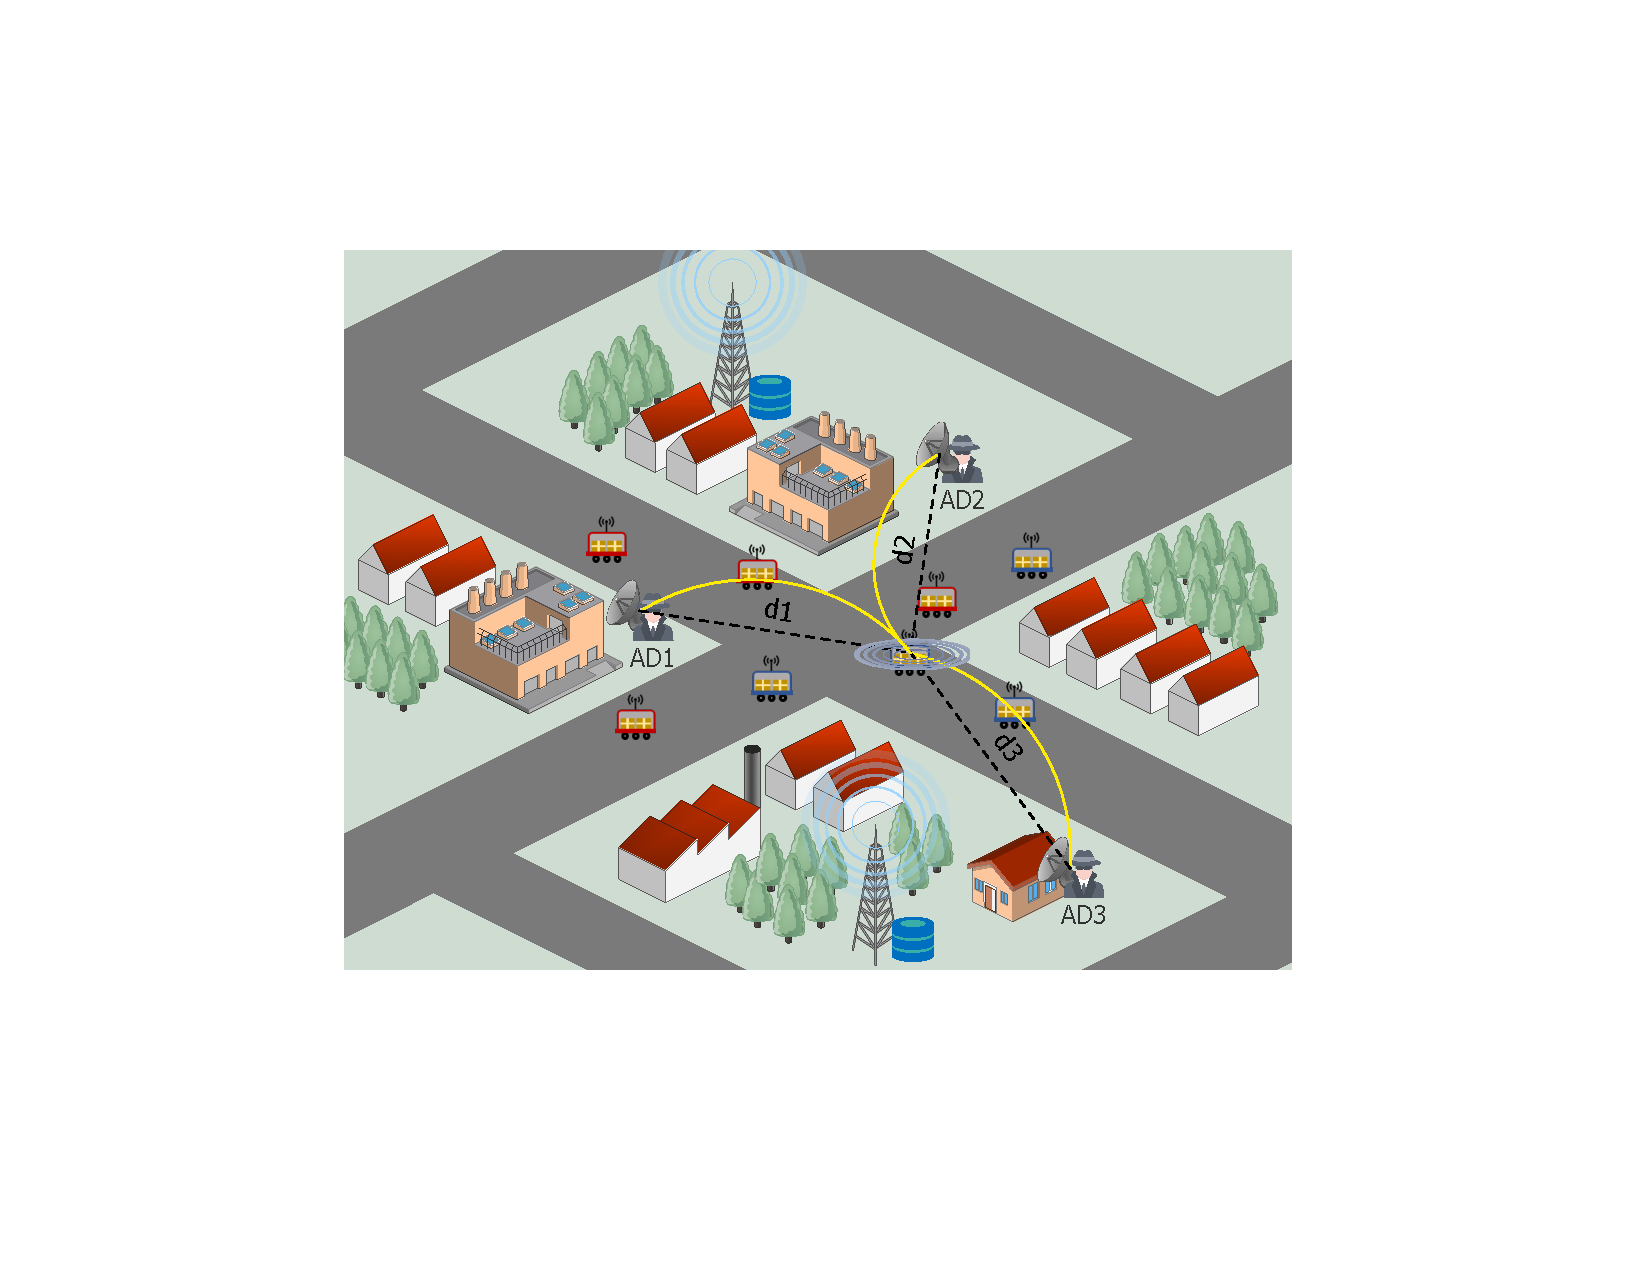
\includegraphics[scale=0.48]{./pic/Diagram22.pdf}
%\caption{An illustration of RSS based adversarial localization attack on an unmanned ground delivery system consisting of robotic vehicles belonging to two companies (differentiated by the colors). $d_1, d_2, d_3$ are distance estimations extracted from RSS measurements at three different positions, and are utilized to localize the target via trilateration technique.}\label{fg:trilate}
%\end{figure}
%
%With the expanding scale of IoT devices, the tremendous industrial data generated has put an increasing demand on bandwidth resources, which poses a significant challenge on the industrial spectrum management. To address the spectrum shortage, database-assisted spectrum access has been introduced where IoT are informed with the dynamic spectrum availability by a geo-location database, and access vacant licensed channels opportunistically \cite{TII-dynamic, TII-game}. The key challenge of dynamic spectrum access remains as how to coordinate the spectrum sharing in a distributed way, so that the mutual interference between devices having access to the same vacant channel can be effectively mitigated \cite{TII-game}. To this end, game theoretic models have been adopted for solving dynamic spectrum access problem, where devices are interpreted as selfish players making channel access decisions strategically to maximize their payoffs \cite{wang2010game}. 
%
%
%In addition to the spectrum scarcity, cyber-physical security remains to be another challenge for reliable operation of IIoT. As a main building block of industrial CPS, IIoT integrates the control, networking and computing components, providing fundamental supports for generation, collection and exchange of security-critical and privacy-sensitive data. The critical importance of IIoT makes itself an attractive and valuable target for cyber-physical attacks \cite{securitysuvey}. While extensive studies have been concerning the cyber-attacks and corresponding defenses, relatively less attention has been paid to the physical-layer attacks in IIoT. 
%%Among the many potential security attacks, the adversarial localization attack utilizing physical-layer information of victim's signals has been shown to be effective   []. 
%As a key vulnerability, the geo-location information of IoT devices, once being compromised, would put the device into great danger, which is extremely harmful for the reliability and safety of IIoT system. 
%
%In this study, we consider a practical RSS based adversarial localization attack that has been shown to be effective in pinpointing wireless IoT devices \cite{LocalizationLi}. 
%As illustrated in Fig. \ref{fg:trilate}, given a few RSS measurements collected within the vicinity of the victim, the adversary can easily carry out the localization attack using existing triangulation technique \cite{TOARSS}. Compared with localization approaches using other physical-layer informations (e.g., time of arrival (TOA), time difference of arrival (TDOA), angle of arrival (AOA) \cite{Gezici:08}), RSS based localization requires neither complex hardware nor active communication with the victim, which can be easily implemented by the adversary in practice.

%Many efforts have been made on developing countermeasures to mitigate physical-layer localization attacks, such as deploying directional antenna to limit transmission coverage \cite{antenna} and creating ghost locations to misguide adversaries via device-level cooperation \cite{Sangho12}. However, these approaches might be costly and difficult for widely system deployment, given the fact that IoT devices are generally of small size with limited computation and energy resources. Therefore, we consider using the light-weight power perturbation approach to combat the RSS based localization attack \cite{Jiang07}. The main idea behind is to add random noise to the transmission power level of IoT devices, with the aim to effectively lower the adversaries' localization accuracy \cite{EI10}. 
%
%Despite its practicability and effectiveness, the random power perturbation approach would result in inaccurate interference evaluation at IoT devices, which inevitably incurs performance degradation (e.g., throughput reduction) to the spectrum sharing system. Thus motivated, the goal of this study is to develop an effective spectrum sharing scheme in IIoT that can at the same time protect device's location privacy via transmission power perturbation. 
%
%Following \cite{Chenjournal}, we formulate the privacy-preserving spectrum access problem as a stochastic game where IoT devices update their channel selection choices dynamically with the objective of maximizing their utilities, as will be defined in Section \ref{sec:system-model}. 
%%To preserve the location privacy, IoT devices are allowed to judiciously add random noise to their transmission power levels.

为了在随机功率扰动影响下求解信道选择博弈的相关均衡(本文中简称为CE),本研究设计了一种双时间尺度的分布式学习算法。具体而言,在相对较大的时间尺度内,每个移动用户根据{\kaishu 带修正的无悔规则}\cite{Hart_areinforcement}来对其信道选择策略进行迭代。而在相对较小的时间尺度上,用户通过一个效用学习的动态过程不断更新其对于社交群体效用的估计,以解决由功率扰动引入的群体效用所含的随机噪声,提高在较大时间尺度上策略学习的效果。我们的分析指出,当学习过程的时间尺度满足一定温和的条件时,用户的联合决策的经验概率分布可以收敛于CE的集合。仿真结果验证得出,在随机功率扰动下,我们的双时间尺度学习算法优于仅使用信道选择策略自适应的单时间尺度学习算法。同时,评估结果表明我们所提出的双时间尺度学习算法有助于实现系统吞吐量和位置隐私保护之间的权衡。
%To solve for the CE of the channel selection game under the impact of random power perturbation, in this study we devise a two-timescale distributed learning algorithm. Specifically, at a slower timescale, each IoT device evolves her channel selection strategy according to a \emph{modified regret-based rule} \cite{Hart_areinforcement} using the locally maintained estimated utility. At a relatively faster timescale, the estimated utility keeps being updated via a learning process to address the randomness introduced by the power perturbation, which facilitates more effective strategy learning at the slower timescale. We show that under mild conditions on the learning timescales, the empirical frequency of users' joint actions converges to the set of CE. The simulation results show that, under the random power perturbation, our two-timescale learning algorithm outperforms the single timescale learning algorithm involving only the strategy adaptation of channel selection, which corroborates that the proposed two-timescale learning algorithm helps strike a balance between the system throughput and location privacy.

与大多数现有工作不同,本文的问题建模与求解过程中将频谱管理与用户位置隐私保护紧密地结合在一起。
%\cite{Bennis13}启发了提出的两时尺度学习算法的思想,该研究使用基于增强学习的算法研究了分散式小蜂窝网络中的干扰缓解。
%与我们较为相关的工作是\cite{ZhangGlobe},该文中作者使用博弈论模型研究了在具有社交意识的动态频谱访问情况下的位置隐私保护。在这项研究中,我们考虑了一个不同的均衡标准(即相关均衡),该标准通过放宽对玩家渠道选择策略的独立性假设来概括\cite{ZhangGlobe}中考虑的纳什均衡。此外,物联网设备旨在适应基于后悔规则\cite{Hart00asimple}的策略,而不是\cite{ZhangGlobe}中使用的随机虚拟对弈动态过程。
综上,我们的工作包含以下几点贡献:
%Summarizing, we have made the following contributions:
\begin{itemize}
\item 我们从双重网络外部性的视角阐释了频谱共享网络中存在的物理信号干扰(负网络外部性)与社交效应(正网络外部性),并通过社交群体效用函数的定义对两种效应进行了刻画。
\item 我们指出了在数据库辅助频谱接入系统中的基于RSS的位置隐私攻击隐患,并考虑了一种轻量级的功率扰动方法来降低隐私攻击者的定位精度。
%We identify the issue of RSS based adversarial localization attacks against IoT devices in database-assisted spectrum access, and consider a light-weight power perturbation approach to reduce the localization accuracy.
\item 我们通过一个隐私保护下信道选择博弈的建模来研究在动态频谱接入系统中进行位置隐私保护的问题。我们允许移动设备使用添加有扰动项的传输功率水平进行信号传输并策略性地做出信道选择决策以最大化其社交群体效用。
%We jointly study the dynamic spectrum access and location privacy protection by formulating a privacy-preserving channel selection game where IoT devices use perturbed transmission power level and strategically make channel selection decisions to maximize their utilities.
\item 我们提出了一种基于无悔学习规则的双时间尺度学习算法。该算法弱收敛于相关均衡集合,并且在用户使用随机功率扰动的情况下可以获得优于单一时间尺度学习算法的系统吞吐量指标。
%We propose a two-timescale learning algorithm based on regret learning rule, which converges weakly to the set of correlated equilibria and is shown to outperform the single timescale learning approach in alleviating the system throughput degradation from random power perturbation.
\end{itemize}
本章的其余部分安排如下。第\ref{sec:model}节首先介绍了隐私保护下具有社交意识的频谱共享的系统模型。第\ref{sec:game}节给出了用于频谱共享的SGUM博弈建模,并介绍了{\kaishu 无悔学习规则}(No-regret learning rule)。接下来,第\ref{sec:algorithm}节提出了隐私保护下频谱共享的双度尺度无悔学习算法,并在第\ref{sec:simulation}节中对算法的表现进行了评估。最后,第\ref{sec:con}节对本章进行了总结。
%The remainder of the paper is organized as follows. We first discuss the related work in Section \ref{sec:related}. In Section \ref{sec:model}, we describe the system model of socially-aware privacy-preserving spectrum sharing scheme. In Section \ref{sec:game}, we present the SGUM game formulation for spectrum sharing and introduce the no-regret based learning rule. Then we describe the two-time-scale regret-based learning algorithm for privacy-preserving spectrum sharing in Section \ref{sec:algorithm}, followed by the Section \ref{sec:simulation} which evaluates the effectiveness of the proposed algorithm. Finally, we conclude the paper in Section \ref{sec:con}.

%\section{研究现状}\label{sec:related}
%%Spectrum management techniques have been widely adopted into smart IIoT designs to meet the high QoS requirement for data communication, which helps to establish strong interconnection among industrial sensor, actuators and systems. For instances, Cao {\em et al.} in \cite{CaoCR} explored opportunistic accessibility of multiple channels to enhance the state estimation performance in a CPS with linear state dynamics. In \cite{TIICR}, Chiwewe {\em et al.} provided an overview of different techniques for spectrum management in cognitive radio based industrial wireless sensor network, and also explored the application of game theoretic modeling for spectrum sharing schemes.
%
%
%
%%We start with a brief review on related work on socially-aware spectrum sharing. Xing \emph{et al.}~proposed to use anthropological models in human society to enhance the performance of cognitive radio networks \cite{xing2008human}. Li \emph{et al.} \cite{li2011propagation} carried out social network analysis of the social behavior in cognitive radio networks. Another common approach for spectrum sharing based on social interactions is to model secondary users' interactions as noncooperative game (e.g., \cite{wang2010game} and many others) assuming they are \emph{selfish yet rational}. Notably, Chen \emph{et al.} \cite{chen2012spatial} developed a spatial spectrum access game framework to model the competitive spectrum access among the secondary users by taking the spatial reuse effect into account. 
%
%%Nie \emph{et al.} \cite{nie2005adaptive} designed a self-enforcing distributed spectrum access mechanism based on potential games. 
%%Law \emph{et al.} in \cite{law2009price} studied the system performance degradation due to the competition of secondary users in a distributed spectrum access game. 
%
%
%%Along a different avenue, industrial cyber-physical security issues have recently garnered much attention by both industry and academic communities, with great efforts focusing on the cyberattacks over industrial CPS \cite{securitysuvey}. In \cite{CPSsecurity}, the authors proposed a CPS security framework that distinguished the cyber, cyber-physical, and physical components in a CPS system, and surveyed over both potential and reported attacks as well as existing solutions. Particularly, in \cite{smartmeter}, the authors focused on the data privacy vulnerability of smart meters in smart grid system, and provided a thorough discussion on the state-of-the-art mitigation solutions. And in \cite{smartcity}, the authors discussed the the security and privacy challenges within emerging smart city applications such as intelligent healthcare and transportation system. 
%
%%By contrast, the adversarial localization attack considered in this study is a typical physical-layer attack targeting on wireless sensor networks in general \cite{Jiang07}. To combat such threats, one main approach is to obfuscate the physical information of the transmitted signal that can be potentially utilized by adversaries to infer the users' locations. In \cite{Jiang07} and \cite{EI10}, mobile devices were designed to strategically reduce their transmission power so as to reduce the number of adversaries that can collaboratively carry out RSS-based localization attacks, or to degrade the accuracy of the adversarial localization. In \cite{Ting11}, 
%%Oh {\em et al.} \cite{Sangho12} and Taha {\em et al.} \cite{Xuemin13} proposed solutions that create fake locations to mitigate the RSS-based localization attacks. 
%
%近些年来,有关于无线网络中位置隐私保护的相关问题获得了极大的关注。
%%Along a different avenue, location privacy has recently garnered much attention with great efforts focusing on privacy protection  at the application layer. 
%%The major approaches include location obfuscation (e.g., \cite{Agrawal:Privacy}), anonymization (e.g., \cite{Beresford:Mix, Gongjournal, Shin:AnonySense}), differential privacy (e.g., \cite{Dwork:Differential}) and cryptographic-based transformation (e.g., \cite{Ghinita:Private, Khoshgozaran:Blind}), each being suitable for different type of applications. 
%%Location-obfuscation schemes perturb users' location information by adding random noises to their locations. In anonymization, there are two different approaches: pseudonym (e.g., \cite{Beresford:Mix}) and $k$-anonymity (e.g., \cite{Shin:AnonySense}). The former decouples the link between users' real identity and their location information, while the latter ensures that there are at least $k$ users whose locations are indistinguishable. Differential privacy protects the information of each individual in the database while publishing statistical information (e.g., average) about the database. Cryptographic-based transformation encrypts users' location information to make it confidential. 
%%Nevertheless, these application-layer solutions have very limited effectiveness against the physical-layer location privacy attacks in wireless networks, which aim at localizing users based on the measurements of their transmitted signals.
%在一些网络物理层的位置隐私攻击模型中,攻击者主要利用信号的物理信息来推断用户的位置。因而使传输信号的物理信息变得模糊成为了一种防御物理层位置隐私攻击的主要手段。在\cite{Jiang07}和\cite{EI10}中,移动设备通过策略性地降低其传输功率,从而可以有效减少可参与协作进行RSS定位的攻击者数量,或降低攻击者RSS定位的准确性。 Wang等\cite{Ting11}则着重于定向天线的设计,以解决物理层位置隐私攻击的问题。Gao等\cite{location}所应用的位置隐私保护措施与本文中所使用的较为接近。然而与本文所考虑的基于RSS的定位攻击不同,\cite{location}中考虑的是通过推断目标用户所使用的信道来判断其位置。因而目标用户可以通过选择最有利的信道来缓解隐私攻击的威胁。
%%As for the physical-layer location privacy attacks in wireless networks, one main approach is to obfuscate the physical information of the transmitted signal that can be potentially utilized by adversaries to infer the users' locations. In \cite{Jiang07} and \cite{EI10}, mobile devices are allowed to strategically reduce their transmission power so as to reduce the number of adversaries that can collaboratively carry out RSS-based localization attacks, or to degrade the accuracy of the RSS-based localization. Wang {\em et al.} focused on the design of directional antenna to address the physical-layer location privacy attacks. In \cite{location}, Gao {\em et al.}  considered the location privacy protection in a cognitive radio network similar to ours. While instead of the RSS-based attack, they considered an attack model that inferred a secondary user's location through her used channels, and the threat was mitigated by choosing channels in favor of the most stable ones.
%
%与大多数现有工作不同,本文我们共同考虑频谱管理和位置隐私保护。\cite{Bennis13}启发了提出的两时尺度学习算法的思想,该研究使用基于增强学习的算法研究了分散式小蜂窝网络中的干扰缓解。也许与我们最相关的工作是\cite{ZhangGlobe},它使用博弈论模型研究了在具有社交意识的动态频谱访问情况下的位置隐私保护。在这项研究中,我们考虑了一个不同的均衡标准(即相关均衡),该标准通过放宽对玩家渠道选择策略的独立性假设来概括\cite{ZhangGlobe}中考虑的纳什均衡。此外,物联网设备旨在适应基于后悔规则\cite{Hart00asimple}的策略,而不是\cite{ZhangGlobe}中使用的随机虚拟游戏动力学。
%%Different from most of the existing works, in this paper we jointly consider the spectrum management and locational privacy protection. The idea of the proposed two-timescale learning algorithm is inspired by \cite{Bennis13}, which studied the interference mitigation in decentralized small-cells networks using a reinforcement learning based algorithms. Perhaps The most related work to ours is \cite{ZhangGlobe}, which investigated the location privacy protection under the scenario of socially-aware dynamic spectrum access by using game theoretic modeling. In this study, we consider a different equilibrium criteria (i.e., correlated equilibrium) which generalizes the Nash equilibrium considered in \cite{ZhangGlobe} by relaxing the independence assumption on the players' channel selection strategies. In addition, the IoT devices are designed to adapt strategy following the regret-based rule\cite{Hart00asimple} instead of the Stochastic Fictitious Play dynamics used in \cite{ZhangGlobe}. 
%
%%\section{System Model for Locational Privacy Preserving Spectrum Sharing}\label{sec:model}
\section{位置隐私保护下的频谱共享系统模型}\label{sec:model}


%\subsection{Basic Setting}\label{sec:system-model}
\subsection{基本设置}\label{sec:system-model}
根据FCC\cite{FCCApril52012}的规定,在数据库辅助频谱访问中,每个空白用户将首先向数据库发送频谱访问请求,然后数据库将向该用户显示在特定位置处空闲的TV信道。我们考虑这样的一个由主信道(例如电视频道)频谱集合$\mathcal{M}athcal{A}=\{1,2,\cdots,M\}$组成的频谱接入网络。在这个网络中有一组次级用户$\mathcal{M}athcal{V}=\{1,2,\cdots,N\}$会去尝试在信道未被主用户占用的情况下访问这些空闲的信道。具体来说,每个用户$n\in\mathcal{M}athcal{V}$可以访问数据库公布的一个可用信道子集$\mathcal{M}_n\subseteq\mathcal{M}athcal{A}$。显然,如果次级用户之间没有适当的协调,则可能会发生信道使用的冲突,且所产生的信道干扰会严重影响网络的性能。 {\kaishu 因此,在存在时变信道占用和干扰的环境中,数据库辅助频谱接入可以被归结为次级用户之间的动态信道分配。}
%According to the recent ruling by FCC \cite{FCC}, in database-assisted spectrum access, each white-space user will first send a spectrum access request to a database, and the database will reveal the vacant TV channels at a particular location to that user. We consider such a spectrum access network with a set $\mathcal{M}athcal{A}=\{1,2,\cdots,M\}$ of primary channels (e.g., TV channels). And a set $\mathcal{M}athcal{V}=\{1,2,\cdots,N\}$ of secondary users (i.e., IoT devices) try to access these channels when the channels are not occupied by licensed users. In particular, each user $n\in\mathcal{M}athcal{V}$ can access a subset of available channels $\mathcal{M}_n\subseteq\mathcal{M}athcal{A}$, as revealed by the database. Apparently, without proper coordination among secondary users, the conflict on channel usage may occur, and the generated interference could severely degrade the network performance. {\em Accordingly,  database-assisted spectrum access boils down to the dynamic channel allocation among secondary users, in a time-varying channel occupancy and interference environment.}
\begin{figure}[!t]
%\hspace{-0.35cm}
\centering
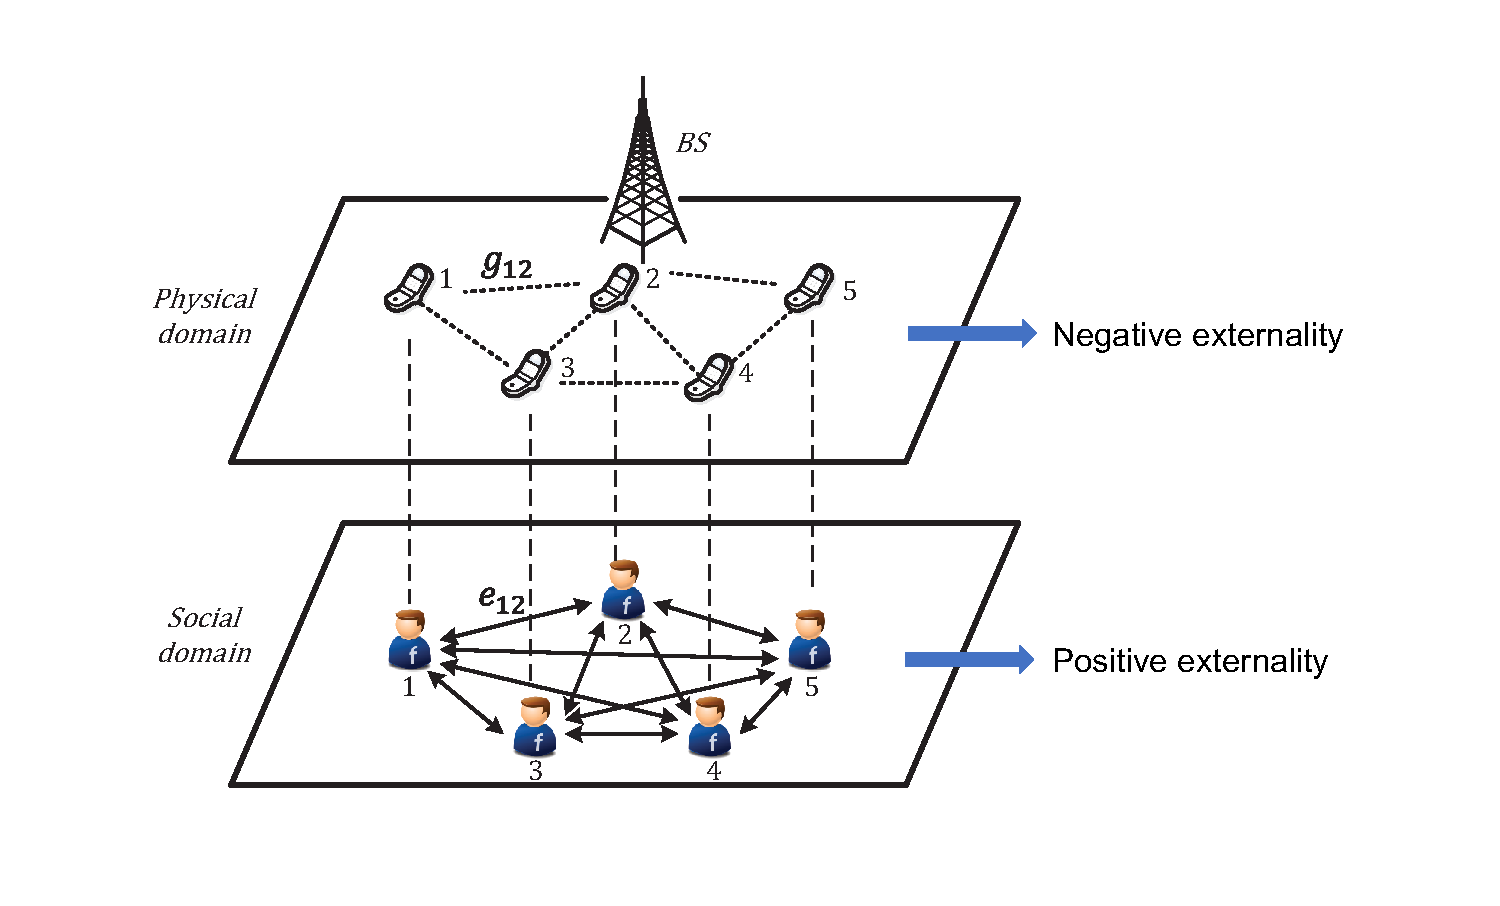
\includegraphics[scale=0.64]{./pic/sysfig11.pdf}
\caption{认知无线电网络的社交域-地理域说明}\label{fg:domain}
\end{figure}

参照文献\cite{Chenjournal},我们考虑一个具有社交意识的认知无线电网络(如图\ref{fg:domain}所示),其中每个次级用户在选择频道时都考虑了地理位置和社交关系所决定的双重网络外部性的影响。
%Following \cite{Chenjournal}, we consider a socially-aware cognitive radio network (as illustrated in Fig. \ref{fg:domain}), where each secondary user takes both physical and social aspects into account during channel selection. 
%In particular, the social relationships among secondary users are leveraged to facilitate cooperation in spectrum sharing. 
一方面,由于数据传输产生的信道干扰,次级用户在地理域中耦合,并希望通过减弱干扰来增加其传输效用。而接入同一信道的用户越多,单一用户的效用越差(负网络外部性)。另一方面,次级用户通过他们之间的社交联系在社交域中相互耦合。由于用户的大部分通信流量产生于同社交好友之间的互动,因此社交好友通信吞吐量的提升对于用户个人的效用带来非直接的正向影响(正网络外部性)。对于具有社交意识的次级用户,在进行通信时考虑与其有社交联系的其他次级用户的效用,将形成一种双赢的局面。
%On the one hand, secondary users are coupled in the physical domain due to the interference relationship in data transmissions, and would like to increase their utilities through interference mitigation. On the other hand, secondary users are coupled in the social domain via the social ties among them. It would be a win-win case for socially-aware secondary users to consider the utilities of those users having social trust with him (her).

我们使用一个信道干扰模型来刻画设备之间的地理位置上的耦合。具体来说,我们令$a_n\in\mathcal{M}_n$表示为用户$n\in\mathcal{M}athcal{V}$所访问的信道,并将其通信链接上的信道增益表示为$g_{nn}^{a_n}$。然后我们令$g_{mn}^{a_n}$表示用户$m\in\mathcal{M}athcal{V}$和用户$n$的通信链路之间在信道$a_n$上的干扰增益。我们用$N_{a_n}$表示用户$n$的链路在信道$a_n$上的噪声,对应的信噪比(SINR)$\gamma_n(P_n)$可以表示为
%To capture the physical coupling among devices, we assume a physical interference model. Specifically, we denote $a_n\in\mathcal{M}_n$ as the channel that user $n\in\mathcal{M}athcal{V}$ have accessed, and denote the channel gain on her communication link as $g_{nn}^{a_n}$. We then let $g_{mn}^{a_n}$ denote the channel gain of $a_n$ over the interference link between user $m\in\mathcal{M}athcal{V}$ and user $n$. The noise of channel $a_n$ on the link of user $n$ is denoted as $N_{a_n}$. The Signal-to-Interference and Noise Ratio (SINR) $\gamma_n(P_n)$ of user $n$ can be written as
\begin{equation}
\small
\gamma_n(P_n)=\frac{P_{n}g_{nn}^{a_n}}{\sum_{m\in \mathcal{M}athcal{V}/\{n\}}P_{m}g_{mn}^{a_n}\mathcal{M}athds{1}_{\{a_m=a_n\}}+N_{a_n}},
\end{equation}
其中$P_n$是用户$n$使用的传输功率;当用户$m$和用户$n$访问同一信道时,指示函数$\mathcal{M}athds{1}_{\{a_m = a_n\}}$等于1,反之等于零。我们用$W$表示带宽,并将功率水平为$P_n$时的吞吐量定义为用户$n$的个体效用函数,即
%where $P_n$ is the transmission power used by user $n$; the indicator function $\mathcal{M}athds{1}_{\{a_m=a_n\}}$ is equal to 1 when user $m$ and user $n$ access to the same channel (i.e., $a_m=a_n$), and zero otherwise. We let $W$ denote the bandwidth, and define the individual utility of user $n$ as her throughput with power level $P_n$,
\vspace{-0.2cm}
\begin{equation}\label{indiu}
U_n=W\log[1+\gamma_n(P_n)].
\end{equation}

我们使用无向社交图$G^S=\{\mathcal{M}athcal{V},E\}$来对用户之间的社交耦合进行建模。其中每个顶点对应于集合$\mathcal{M}athcal{V}$中的一个用户,用图中无向的边表示用户之间的社交关系。特别的,我们对于联结任意两个用户$n$和$m$的边赋予一个权重$e_{nm}\in [0,1]$来量化两个用户之间社交关系的亲密程度。此外,我们所定义的权重具有以下特性:$e_{nm}=e_{mn},e_{nn}=1, \forall n,m\in\mathcal{M}athcal{V}$。
%The social coupling among users is modeled by using an undirected social graph $G^S=\{\mathcal{M}athcal{V},E\}$, with each vertex corresponding to a user within set $\mathcal{M}athcal{V}$, and undirected edges indicating the social relationship among users. In particular, we assign a weight $e_{nm}\in [0,1]$ to the edge connecting two arbitrary users $n$ and $m$ to quantify the closeness of the social relationship between the two users. Further, the edge weights have the following characteristics: $e_{nm}=e_{mn},e_{nn}=1, \forall n,m\in\mathcal{M}athcal{V}$.
%\subsection{Social Group Utility Maximization (SGUM) for Spectrum Access}
%As hand-held devices are carried by human beings, the social relationships among users can be leveraged to enable such collaborations among users. Intuitively, by taking into consideration of the social aspect, users are expected to select channels more wisely instead of in a fully selfish manner. 
我们使用社交群体效用模型来刻画存在社交联系的设备之间潜在的社交耦合,在这里,我们定义用户$n$的社交群体效用函数为
\vspace{-0.2cm}
\begin{equation}\label{sgu}
S_n=U_n+\sum_{m\in \mathcal{M}athcal{V}/\{n\}}e_{nm}U_m.
\end{equation}
该定义中用户的个体效用刻画了用户间的{\kaishu 负网络外部性}影响,而对于社交好友个体效用的加权求和则刻画了用户之间的{\kaishu 正网络外部性}效应。
%。直观地,$e_n$的值越大,设备$n$与其所关联的群体之间的社交联系越强。
%We use such a group utility model to capture the underlying social coupling among homogeneous IoT devices within the same group. Intuitively, the larger the value of $e_n$, the stronger the social connection that device $n$ has with respect to the group she is associated with.


%\subsection{Random Power Perturbation against RSS-based Location Privacy Attack}\label{sec:privacy-model}
\subsection{针对基于RSS的位置隐私攻击的随机功率扰动}\label{sec:privacy-model}
\subsubsection{基于RSS的位置隐私攻击}
在这项研究中,我们考虑了一个物理层攻击者模型,该模型采用基于接收信号强度(RSS)的定位技术来获取目标用户的位置隐私。基于RSS的定位可以捕获传输的信号,并可以根据信号传播模型\cite{Jiang07,EI10}建立距离与RSS之间的映射。每个攻击者可以采集一系列目标用户发射信号的RSS电平\footnote{例如,通过采集信号RSS并结合RF指纹技术\cite{TIEYuanchao},信号接收者可以通过分析信号模拟分量中的瑕疵来识别无线网卡。},并使用通过最大似然估计\cite{RSSguang}获得距离的估计。
%In this study, we consider a PHY-layer adversary model that employs the Received Signal Strength (RSS) based localization technique to compromise target users' location privacy. RSS-based localization captures the transmitted signal and can establish the mapping between the distance and the RSS according to the signal propagation model \cite{Jiang07,EI10}. As illustrated in Fig. \ref{fg:trilate}, each adversary can collect a sequence of RSS levels of the transmitted signal from the target user\footnote{For instance, through the RF fingerprint technique\cite{TIEYuanchao}, a receiver can identify a wireless card by analyzing imperfections in the analog components of the signal.}, and obtain an estimation of the distance using via Maximum Likelihood estimation \cite{RSSguang}. 
%According to the propagation model (e.g., the log-normal model), each adversary can obtain an estimation of the distance between the target user and herself.  sequence of RSS measurements
然后,攻击者可以通过使用一组距离估计结合其自身地理位置使用三角测量的方法近似地确定目标用户的位置。
%Then an approximate location of the target user can be jointly determined by a trilateration using a set of distance estimations and the corresponding physical positions of the adversary.


\subsubsection{传输功率随机扰动}
为了对抗基于RSS的位置隐私攻击,我们采用了一种本地传输功率随机扰动的方法,旨在增加攻击者定位结果的不确定性\cite{EI10}。为此,每个用户可以动态地随机改变其传输功率水平。攻击者收集到的带有噪声的RSS测量值会有效地扩大目标用户定位的不确定性区域,从而降低定位精度。
%To combat RSS-based location privacy attack, we employ a local random power perturbation approach aiming to introduce uncertainties to adversaries' localization outcome\cite{EI10}. To this end, each user is allowed to dynamically and randomly change her transmission power level on purpose. The noisy measurements of RSS obtained at the adversary could effectively enlarge the uncertainty region of target user's position, which reduces the localization accuracy.

为了避免对主用户的额外干扰,我们限制随机功率扰动分量为负偏值。具体来说,用户$n$扰动后的传输功率可表示为$P_n=p+\Delta p_n$,即常规传输功率电平$p> 0$和扰动项$\Delta p_n$的加和。扰动项可被表示为一个服从单边截断指数分布的随机变量,其概率密度函数的表达式为
%To avoid extra interference to the primary users, we restrict the random power perturbation component to be negative biased. Specifically, the perturbed transmission power of user $n$ is given by $P_n=p+\Delta p_n$, which is the sum of the regular transmission power level $p>0$ and a perturbation term $\Delta p_n$, generated following one-side truncated exponential distribution whose \emph{pdf} is given as
\begin{equation}\label{eq:noise}
%\small
f(\Delta p_n|b,\bar{p})=\frac{\frac{1}{b}\exp(\Delta p_n/b)}{1-\exp(\bar{p}/b)},~\Delta p_n\in(-\bar{p},0],
\end{equation}
其中$\bar{p}$表示最大扰动量。当扰动超出该范围时,将导致SINR过小而不满足正常数据传输的要求。参数$b>0$则刻画了用户指定的一个“平均”功率扰动水平,我们将在节\ref{sec:simulation}中对其做进一步讨论。

%with $\bar{p}$ denotes the maximum perturbation level beyond which the SINR of IoT device might be unacceptable for normal data transmission. The parameter $b>0$ characterizes the ``expected'' power perturbation level specified by the user, as will be further discussed in Section \ref{sec:simulation}.

%\section{Socially-aware Privacy-preserving Spectrum Sharing}\label{sec:game}
\section{隐私保护下带有社交意识的频谱共享}\label{sec:game}
在本节中,我们将频谱共享问题转换为社会团体效用最大化(SGUM)博弈,并介绍了无悔学习规则,该规则可以以分布式方式计算非合作博弈的相关均衡。
%In this section, we cast the spectrum sharing problem as a social group utility maximization (SGUM) game, and introduce the no-regret matching rule, which can calculate the correlated equilibrium of a non-cooperative game in a distributed manner.

%\subsection{Social Group Utility Maximization (SGUM) Game for Spectrum Sharing}\label{sec:SGUM}
\subsection{频谱共享中的社交群体效用最大化(SGUM)博弈}\label{sec:SGUM}
在我们的研究中,我们将系统中的每一对接收发射端视为一个用户,他们之间存在持续的策略性的交互,旨在从长远来看最大化他们各自的社交群体效用。
为此,我们将隐私保护下的频谱共享问题建模为一个社交群体效用最大化(SGUM)博弈,每一个用户对应于博弈中的一个玩家\footnote{是本章中,术语上“用户”和“玩家”可以互换。}。
%In our study, all the transmitter-receiver pairs in the system are modeled as self-interested users interacting strategically and repeatedly with each other, aiming to maximize their social group utilities in the long run. 
%To this end, we formulate the privacy-preserving spectrum sharing problem as a \emph{social group utility maximization (SGUM) game} with the players corresponding to the users\footnote{We use the terms ``user'' and ``player'' interchangeably throughout the paper.}.
%In addition, each $TR$ will actively perturb her transmission power in order to mitigate the threat of RSS based location privacy attack.
每个玩家$n\in\mathcal{M}athcal{V}$的行为空间在这里被定义为用户$n$可以接入的可用信道集合$\mathcal{M}_n$。我们令$\A=(a_1,a_2,\cdots,a_N)\in\mathcal{M}$表示所有用户的联合频谱接入选择方案,其中$\mathcal{M}\triangleq\prod_{n=1}^N\mathcal{M}_n$。
%The action space of each player $n\in\mathcal{M}athcal{V}$ is the set of available channels $\mathcal{M}_n$ that user $n$ can access. We let $\A=(a_1,a_2,\cdots,a_N)\in\mathcal{M}$ denote the joint spectrum access profile of all the users, where $\mathcal{M}\triangleq\prod_{n=1}^N\mathcal{M}_n$. 
%Since the observed social group utility is noisy due to the power perturbation implemented by each user, it makes more sense for each user to target on maximizing its 
为了便于评估每个用户的长期社交群组效用期望,我们令$\Delta\mathcal{M}_n$表示用户$n$的混合策略空间,并令$\pi_n=\left(\pi(a_{n,1}),\pi(a_{n,2}),\cdots,\pi(a_{n,|\mathcal{M}_n|})\right)\in\Delta\mathcal{M}_n$表示用户$n$的混合策略。其本质上可看作为是定义在$\mathcal{M}_n$上的一个概率分布,其中$q(a_{n,i})$代表用户选择信道$a_{n,i}$的概率。因此,所有玩家的联合混合策略可以被表示为$\p=(\pi_1,\pi_2,\cdots,\pi_N)\in\Delta\mathcal{M}\triangleq\prod_{n=1}^N\Delta\mathcal{M}_n$,而按照管理除用户$n$外的其他玩家的联合策略可以表示为$\p_{-n}=(\pi_1,\cdots,\pi_{n-1},\pi_{n+1},\cdots,\pi_N)$ 。我们进一步令$\pi(\A)$表示联合决策$\A\in\mathcal{M}$在博弈中出现的概率。


%To facilitate the evaluation of each user's long-term expected group utilities, we denote $\Delta\mathcal{M}_n$ as the mixed strategy space of user $n$, and let $\pi_n=\left(\pi(a_{n,1}),\pi(a_{n,2}),\cdots,\pi(a_{n,|\mathcal{M}_n|})\right)\in\Delta\mathcal{M}_n$ denote user $n$'s mixed strategy, a probability distribution over $\mathcal{M}_n$ with $q(a_{n,i})$ representing the probability of selecting the channel $a_{n,i}$. It follows that the joint mixed-strategy over all players is $\p=(\pi_1,\pi_2,\cdots,\pi_N)\in\Delta\mathcal{M}\triangleq\prod_{n=1}^N\Delta\mathcal{M}_n$, and the joint strategy of players excluding user $n$ can be denoted as $\p_{-n}=(\pi_1,\cdots,\pi_{n-1},\pi_{n+1},\cdots,\pi_N)$ by convention. We further denote $\pi(\A)$ as the probability of joint action $\A\in\mathcal{M}$ being played. 

基于以上模型,我们将隐私保护下的频谱共享问题视为一个非合作信道选择博弈,用一个三元组$\Gamma=\left(\mathcal{M}athcal{V},\Delta\mathcal{M},\{S_n\}_{n=1}^N\right)$来表示,博弈中每个玩家旨在最大化自身的期望社交群体效用。我们研究中考虑的均衡标准是{\kaishu 相关均衡(Correlated Equilibrium)}。由于相关均衡允许不同玩家的之间的策略存在相关性,因此可被看做是{\kaishu 纳什均衡(Nash Equilibrium)}的一个泛化。数学上来看,一个相关均衡对应一个凸多面体,凸面体的极值点对应于纳什均衡。因此,通常系统可以在达到相关均衡时比达到纳什均衡时获得更好的总体性能。
%Summarizing, we cast the privacy-preserving spectrum sharing problem as a non-cooperative game denoted by a 3-tuple $\Gamma=\left(\mathcal{M}athcal{V},\Delta\mathcal{M},\{S_n\}_{n=1}^N\right)$. The equilibrium criteria considered in our study is the \textsl{correlated equilibrium}, which generalizes the Nash equilibrium by permitting players' strategies to be dependent. Mathematically, a correlated equilibrium is a convex polytope with its extrema points corresponding to the set of Nash equilibria. Thereby, in general, a better overall performance can be achieved under the correlated equilibrium than that under a Nash equilibrium. 
我们在下面给出相关均衡的正式定义。
%The formal definition of correlated equilibrium is given below.


\begin{df}[相关均衡]
我们称定义在$\Delta\mathcal{M}$上的概率分布$\pi^*$为信道选择博弈$\Gamma$的一个相关均衡(CE),如果$\forall n\in\V$,$\forall a_{n,i},a_{n,j}\in\mathcal{M}_n$,社交群体效用$S_n$满足以下不等式,
%A probability distribution $\pi^*$ on $\Delta\mathcal{M}$ is a socially-aware correlated equilibrium (CE) of game $\Gamma$ if, $\forall n\in\V$, $\forall a_{n,i},a_{n,j}\in\mathcal{M}_n$, the expected group utility satisfies the following,
\begin{equation}
\sum_{\textbf{a}\in\mathcal{M}:a_n=a_{n,i}}\pi^*(\textbf{a})\left[S_n(a_{n,j},\textbf{a}_{-n})-S_n(\textbf{a})\right]\leq0.
\end{equation}
\end{df}

\noindent{\bf 备注}
为了获得对相关均衡更具体理解,我们可以将$\pi^*$看作频谱数据库提供的一个信道接入策略推荐。则对于每个用户而言,假设其他用户都遵循频谱数据库所推荐的相应均衡策略,则同样遵循频谱数据库所推荐的策略会是对于该用户最有利的选择。换句话说,用户不能依靠单方面背离CE推荐的策略获得期望社交群体效用的提升。
%To get a concrete sense of the correlated equilibrium herein, one can view $\pi^*$ as a strategy recommendation provided by the trusted spectrum database. With the implicit assumption that other users' strategies follow the given recommendation, it is of best interest of each user to also follow the recommended strategy. In other words, a user could not obtain a better expected group utility by deviating from the CE unilaterally. 

\begin{thm}(CE的存在性)
信道选择博弈$\Gamma$至少存在一个相关均衡(CE)。
%There exists at least a SCE in the stochastic channel selection game $\Gamma$.
\end{thm}
由于我们的信道选择博弈$\Gamma$中的玩家集合和策略集合都为有限集,因此属于有限博弈的范畴,继而保证存在一个非空的相关均衡集合\cite{Lasaulce2011}。
%Since our channel selection game $\Gamma$ consists of finite player set and action set, it falls into the category of finite game, which is guaranteed to possess a nonempty set of correlated equilibria\cite{Lasaulce2011}.


\subsection{无悔学习规则(No-regret learning rule)}\label{sec:noregret}
在本节中,我们简要介绍无悔学习规则,该规则是为以分布式的方式搜索非合作博弈的相关均衡而提出的\cite{Hart00asimple}。通过此规则,可以使用“遗憾度量”来量化玩家的策略调整所带来的性能收益或损失。
该规则的核心思想是让每个用户从每个特定策略的遗憾中学习,目的是最小化长期的平均遗憾度量。
%In this section, we briefly introduce the no-regret matching rule which is developed for searching a correlated equilibrium of a non-cooperative game in a distributed way\cite{Hart00asimple}. By this rule, a regret measure is used to quantify the performance gain or loss of players' action adjustments. 
%The key idea is to let each user learns the regret of playing each particular action, aiming to minimize the average regret over time. 

具体来说,对于每个用户$n\in\V$,给定其对手的策略$\A_{-n}$,则截止到$t$时刻,其在当前策略$a^t_n=a_{n,i}$与某一其他策略$a_{n,j}\neq a_{n,i}$下的平均群体效用之差为
%Specifically, for each user $n\in\V$, given her opponents' actions $\A_{-n}$, the difference between averaged group utility under current action $a^t_n=a_{n,i}$ and that under any other action $a_{n,j}\neq a_{n,i}$ until time $t$ can be measured as
\begin{align}\label{eq:reg1}
\small
D_n^t&(a_{n,j},a_{n,i})=\nonumber\\
&\frac{\sum_{l\leq t}S_n(a_{n,j},\A^l_{-n})\mathcal{M}athds{1}_{\{a^l_n=a_{n,i}\}}}{t}-\frac{\sum_{l\leq t}S_n(\A^l)\mathcal{M}athds{1}_{\{a^l_n=a_{n,i}\}}}{t},
\end{align}
其中第二项量化了用户$n$在策略$a_{n,i}$下截止到时间$t$时刻的平均群组效用,而第一项表明了如果用户如果在之前每次选择策略$a_{n,i}$时都换为使用策略$a_{n,j}$所能获得的平均群组效用。直观地来说,用户$n$会产生“遗憾”如果一个替代的策略可以带来更高的效用。在这里,我们就用$R^t_n(a_{n,j},a_{n,i})=\mathcal{M}ax\left\{D^t_n(a_{n,j},a_{n,i}),0\right\}$来表示用户因未使用$a_{n,j}$替代$a_{n,i}$所产生的“遗憾”。
%where the second term quantifies the average group utility perceived by user $n$ under action $a_{n,i}$ until time $t$, and the first term indicates the average utility she would have obtained if she had chosen $a_{n,j}$ every time when $a_{n,i}$ was played. Then user $n$'s ``regret'' for not having played action $a_{n,j}$, instead of $a_{n,i}$ in the previous plays, is given as $R^t_n(a_{n,j},a_{n,i})=\mathcal{M}ax\left\{D^t_n(a_{n,j},a_{n,i}),0\right\}$. Intuitively, user $n$ would regret if an alternate action could have brought her higher utility.

根据时间$t$时刻的遗憾度量,用户$n$将根据以下概率调整其策略,
%Based on the regret measures at time $t$, user $n$ adapts her action according to the probabilistic strategy given as follows,
\vspace{-0.3cm}
\begin{equation}\label{eq:st1}
\begin{cases}
q^{t+1}_n(a_{n,j})=\frac{1}{\mathcal{M}u}R^t_n(a_{n,j},a_{n,i}), ~~~~\forall a_{n,j}\in\mathcal{M}_n/\{a_{n,i}\}, \\
q^{t+1}_n(a_{n,i})=1-\sum_{a_{n,j}\neq a_{n,i}}q^{t+1}_n(a_{n,j}).
\end{cases}
\end{equation}
这里,选择某一替代策略$a_{n,j}\in\mathcal{M}_n/\{a_{n,i}\}$的概率正比于相应的遗憾度量$R^{t}_n(a_{n,j},a_{n,i})$。我们设定参数$\mathcal{M}u$为一个较大的值,以确保用户始终会以一定非负的概率维持当前所选择的信道。较大的$\mathcal{M}u$值会降低切换到其他可选信道的概率,因此$\mathcal{M}u$可以被视为一个“惯性”参数。类似的,在算法进行过程中用户不断地更新自己的遗憾度量。
%Here the probability of changing to an alternate action $a_{n,j}\in\mathcal{M}_n/\{a_{n,i}\}$ is proportional to the corresponding regret measure $R^{t}_n(a_{n,j},a_{n,i})$. The parameter $\mathcal{M}u$ is chosen to be a large value to guarantee that there is always a positive probability of remaining at the currently selected channel. A higher $\mathcal{M}u$ lowers the probability of switching to an alternate channel, therefore can be treated as an `inertia' parameter. The algorithm then moves on by users updating their regret measures at time step $t+1$. 
我们令$f^t(\A)\in\Delta\mathcal{M}$表示联合决策$\A\in\mathcal{M}$截止到$t$时刻的经验分布,表示为
%For each joint action $\A\in\mathcal{M}$, we let $f^t(\A)\in\Delta\mathcal{M}$ denote its empirical distribution by time slot $t$, expressed as
\vspace{-0.2cm}
\begin{equation}\label{eq:empi}
%\small
f^t(\A)=\frac{1}{t}\sum_{l\leq t}\mathcal{M}athds{1}_{\{\A^l=\A\}}.
%f^t(\A)=\frac{|l\leq t:\A^l=\A|}{t}.
\end{equation}
%\vspace{-0.2cm}
根据已有结果我们知道,对于一个非合作博弈,如果玩家遵循无悔学习规则来更新其策略,则当$t\rightarrow\infty$时,经验分布$f^t$会以概率1收敛到相关均衡的集合\cite{Hart00asimple}。
%It is well-known that for a non-cooperative game, with players updating their strategies following the no-regret matching rule, the empirical distributions $f^t$ converges (with probability one) to the set of correlated equilibria as $t\rightarrow\infty$\cite{Hart00asimple}. 

当我们尝试直接使用无悔学习规则来求解我们的随机信道选择博弈问题时会遇到了两个主要挑战。
%由于两个挑战的存在使得我们无法直接使用无悔匹配规则来解决我们的随机信道选择博弈。
首先,由于使用了随机功率扰动程序用以保护隐私,每个用户的群体效用会因随机噪声的引入而遭到损坏,这不可避免地导致了遗憾度量的不准确,并可能导致得到的CE实际表现较差。
%There are two challenges that hinders us from directly using the no-regret matching rule in solving our stochastic channel selection game. Firstly, due to the use of random power perturbation procedure, the group utility of each user is corrupted with random noise, which inevitably leads to inaccurate `regret' measurements and possibly problematic CE of the game.

此外,根据(\ref{eq:reg1})的定义,在计算未使用信道$a_{n,j}$所产生的遗憾时,用户$n$需要评估先前每次使用策略$a_{n,i}$时,若使用替代信道$a_{n,j}$所可以获得的社交群体效用$S_n(a_{n,j},\A^l_{-n})$。而这在实际中是不可行的,因为用户并不掌握其他用户的信道选择策略$\A_{-n}$,以及他们的群体效用函数这些系统全局信息。

%$ S_n(a_每次在时间步骤$ l <t $播放动作$ a_ {n,i} $时,$ a_ {n,j} $以下的{n,j},\ A ^ l _ {-n})$这是不可行的,因为用户$ n $不拥有其他用户的单个实用程序功能及其所选通道$ \ A _ {-n} $的全局信息。
%Further, according to (\ref{eq:reg1}), to compute the regret for not having chosen an alternative channel $a_{n,j}$ , user $n$ needs to evaluate her potentially perceivable group utility $S_n(a_{n,j},\A^l_{-n})$ under $a_{n,j}$ every time when action $a_{n,i}$ was played at time step $l<t$, which is infeasible since user $n$ does not possess the global information of other users' individual utility functions as well as their selected channels $\A_{-n}$. 

为了解决这两个挑战,在下一部分中,我们将设计一种双时间尺度的学习算法,通过该算法,用户可以在相对较小的时间尺度上学习其夹带有噪声的社交群体效用,同时在相对较大的时间尺度上通过一种经过修正的无悔规则来调整其信道选择策略。
%To tackle these two challenges, in the next section, we devise a two-timescale learning algorithm, by which users learn their underlying noisy group utilities in the `faster' learning process, while adapting their channel selection strategies following a modified regret-based rule in the `slower' learning process. 

%\section{Distributed Regret-based Learning for Privacy-Preserving Spectrum Sharing}\label{sec:algorithm}
\section{用于隐私保护下频谱共享的分布式无悔学习算法}\label{sec:algorithm}
在本节中,我们将提出一个双时间尺度的用于寻找信道选择博弈的CE的分布式算法,并对算法在温和条件下的长期弱收敛性进行理论上的分析。
%In this section, we introduce the two-timescale distributed algorithm for finding the CE for our channel selection game, and provide a theoretic analysis on the long-run weak convergence of the algorithm under mild conditions. 

\vspace{-0.2cm}

\subsection{双时间尺度无悔学习算法}

如算法\ref{alg:RCS}中所述,我们设计的学习算法包括一个在相对较小和一个相对较大的学习过程。具体地,在较小的时间尺度上,每个用户会持续地在每个时间步长内基于观察到的带有噪声的效用不断更新对应于每个可用信道的群体效用期望。以这些长期更新的期望团体效用为参照,每个用户同时在相对较大的时间尺度上使用无憾学习规则来调整其策略。接下来,我们分别详细介绍两个时间尺度上的学习过程。
%The learning algorithm, as outlined in Algorithm \ref{alg:RCS}, consists of a `faster' and a `slower' learning process. Specifically, on a faster timescale, each user continuously updates the expected group utility corresponding to each available channel given the noisy utility observation at each time step. Calibrating to the maintained expected group utility, each user adapts her strategy by following the regret-based learning rule at the `slower' time scale. In what follows, we elaborate further on `faster' and `slower' learning processes, respectively.

\subsubsection{较小时间尺度上的效用学习}
在较小的时间尺度上,用户$n$持续更新一个向量$\mathcal{M}athbf{\hat{s}^t_n}=\left(\hat{S}^t_n(a_{n,1}),\hat{S}^t_n(a_{n,2}),\cdots,\hat{S}^t_n(a_{n,|\mathcal{M}_n|})\right)$,其中每个元素$\hat{S}^t_n(a_{n,i})$表示在$t$时刻对于信道$a_{n,i}$所对应的群体效用的估计。随着算法的推进,群体效用的估计更新如下式所示
%In the `faster' learning process, user $n$ maintains a vector $\mathcal{M}athbf{\hat{s}^t_n}=\left(\hat{S}^t_n(a_{n,1}),\hat{S}^t_n(a_{n,2}),\cdots,\hat{S}^t_n(a_{n,|\mathcal{M}_n|})\right)$, with each element $\hat{S}^t_n(a_{n,i})$ denoting the estimated group utility under action $a_{n,i}$ at time step $t$. As time evolves, the estimated group utility is updated as follows:
\begin{equation}\label{estimation}
\hat{S}^t_n(a_{n,i})=(1-\lambda^t)\hat{S}^{t-1}_n(a_{n,i})+\lambda^t\mathcal{M}athds{1}_{\{a^t_n=a_{n,i}\}}S^t_n(a_n^t),
\end{equation}
其中$0<\lambda^t<1$表示学习率。具体地,为了得到$S^t_n(a^t_n)$,每个用户$n$首先观测自己受到的干扰并计算个体效用$U^t_n(a^t_n)$,并查询每个用户$m\in\mathcal{M}athcal{N}_n$所获得的效用$U^t_n(a^t_n)$\footnote{两个有社交关系的用户之间的信息交换可以通过一个公共控制信道来完成。},然后根据式(\ref{sgu})进行求和。在每次迭代$t$中,向量$\mathcal{M}athbf{s^t_n}$中只有元素$\hat{S}^t_n(a_{n,i})$会被更新。通过这种效用学习过程,用户$n$可以渐近地形成对期望群体效用的准确评估,从而确保在较大的时间尺度所进行的策略学习最终可以收敛到CE的集合中。
%where $0<\lambda^t<1$ denotes the learning rate. Specifically, for each user $n$, $S^t_n(a^t_n)$ is obtained by first measuring its own received interference $U^t_n(a^t_n)$, querying the $U^t_m$ received by each user $m\in\mathcal{M}athcal{N}_n$ \footnote{The information exchange among two users within a same group could be fulfilled via a common control channel.}, and then conducting the summation according to (\ref{sgu}). Note that at each iteration $t$, only the element $\hat{S}^t_n(a_{n,i})$ of vector $\mathcal{M}athbf{s^t_n}$ is actually updated. Through this recursive utility learning process, user $n$ can asymptotically form accurate evaluation of the expected group utility which ensures that the strategy learning on slower timescale can finally reach the set of CE.
\begin{algorithm}
\caption{双时间尺度分布式学习算法}
\label{alg:RCS}
\begin{algorithmic}[1]
\STATE \textbf{initialization:} 对于每个用户$n$,
\STATE 初始化$\mathcal{M}athbf{s^0_n}$和遗憾度量$R_n^0(a_{n,j},a_{n,i}), \forall a_{n,i}, a_{n,j}\in\mathcal{M}_n$.
\STATE 每个用户$i$以概率$q^0_n(a_{n,i})=\frac{1}{|\mathcal{M}_n|}$随机选择一个信道$a_{n,i}\in\A_n$。
\STATE 初始化学习率$\lambda^0$和$\epsilon^0$;初始化参数$\gamma$.
\STATE \textbf{end initialization}
\FOR {$n\in\mathcal{M}athcal{V}$}
\STATE \emph{效用学习(较小时间尺度):}
\STATE 观测受到的干扰并计算个体效用$U_n^t(a^t_n)$ by (\ref{indiu}).
\STATE 查询社交邻居的个体效用并根据式(\ref{sgu})计算即时社交群体效用$S_{n}^t(a^t_n)$
%Enquiry the individual utility of neighbors and compute instantaneous group utility $S_{n}^t(a^t_n)$ by (\ref{sgu}).
\STATE 基于式(\ref{estimation})更新对于期望群体效用$\hat{S}_{n}^t(a^t_n)$的估计
%Update the estimation of expected utility $\hat{S}_{n}^t(a^t_n)$ by (\ref{estimation}).
\STATE \emph{策略学习(较大时间尺度):}
\STATE 基于式(\ref{eq:insreg})计算即时遗憾$Q^t_n(a_{n,j},a_{n,i})$,基于式(\ref{eq:reg2})计算遗憾度量$D^t_n(a_{n,j},a_{n,i})$。
% according to (\ref{eq:insreg}), and compute the regret measures $D^t_n(a_{n,j},a_{n,i})$ according to (\ref{eq:reg2}).
\STATE 根据(\ref{eq:str2})更新信道选择策略$\{q^t_n(a_n)\}$,并基于$\{q^t_n(a_n)\}$随机选择下一时刻的信道$a^{t+1}_n$
%Update the channel selection strategy $\{q^t_n(a_n)\}$ according to (\ref{eq:str2}), and randomly select a channel $a^{t+1}_n$ based on $\{q^t_n(a_n)\}$.
\STATE $t\leftarrow t+1$.
\ENDFOR
\end{algorithmic}
\end{algorithm}
%\vspace{-0.2cm}

%\subsubsection{Strategy adaptation on a slower timescale}\label{sec:single}
\subsubsection{较大时间尺度上的策略学习}\label{sec:single}
我们对于节\ref{sec:noregret}中所介绍的标准无悔规则进行修正以用于较大时间尺度上的策略学习。
%At the slower timescale, we implement a modified regret-based learning procedure developed based on the standard no-regret rule as introduced in Section \ref{sec:noregret}. 

特别的,每个用户$n$更新其在当前决策$a^t_n=a_{n,i}$与某一其他决策$a_{n,j}\neq a_{n,i}$下的平均群体效用之差如下
%In particular, each user $n$ updates the averaged group utility difference $D^t_n(a_{n,j},a_{n,i})$ between each alternative action $a_{n,j}\in\mathcal{M}_n/\{a_{n,i}\}$ and the current action $a_{n,i}$ recursively as follows,
\begin{equation}\label{eq:reg2}
D^t_n(a_{n,j},a_{n,i})=(1-\epsilon^t)D^{t-1}_n(a_{n,j},a_{n,i})+\epsilon^tQ^t_n(a_{n,j},a_{n,i}),
\end{equation}
其中$Q^t_n(a_{n,j},a_{n,i})\triangleq[S_n(a_{n,j},\A^t_{-n})-S_n(\A^t)]\mathcal{M}athds{1}_{\{a^t_n=a_{n,i}\}}$定义了在时刻$t$使用了决策$a_{n,i}$而不是$a_{n,j}$所产生的即时遗憾。学习率$0<\epsilon^t<1$的取值决定了无悔策略学习的时间尺度,且应当在设置时与$\lambda^t$的值相对应以保证算法收敛到博弈的CE,这一点将在下文进一步讨论。值得注意的是,式(\ref{eq:reg2})是对式(\ref{eq:reg1})的推广,并且当学习率$\epsilon^t=1/t$时可以约简为式(\ref{eq:reg1})。
%where $Q^t_n(a_{n,j},a_{n,i})\triangleq[S_n(a_{n,j},\A^t_{-n})-S_n(\A^t)]\mathcal{M}athds{1}_{\{a^t_n=a_{n,i}\}}$ is defined as the instantaneous regret for not playing actions $a_{n,j}$ instead of $a_{n,i}$ at time $t$. The learning rate $0<\epsilon^t<1$ determines the timescale of the regret-based strategy learning, and should be set in accordance with the value of $\lambda^t$ to guarantee the convergence to the CE, to be discussed next.
%Note that (\ref{eq:reg2}) generalizes (\ref{eq:reg1}) and can reduce to (\ref{eq:reg1}) with learning rate $\epsilon^t$ being set to $1/t$.  

如上一节所提到的,时刻$t$时,在不知道其他用户的决策$\A^t_{-n}$以及他们的个体效用函数的情况下,计算某一替代决策$a_{n,j}\neq a_{n,i}$所对应的效用是非常困难的。
%As mentioned in the previous section, the perceivable utility under an alternate action $a_{n,j}\neq a_{n,i}$ at time $t$, $S_n(a_{n,j},\A^t_{-n})\mathcal{M}athds{1}_{\{a^t_n=a_{n,i}\}}$, is challenging to compute without the knowledge of other users' actions $\A^t_{-n}$ and their individual utility functions.
%\footnote{It is challenging to directly calculate the regret since the computation of group utility requires the information about group neighbors' individual utilities, which is difficult to get in practice.}. 
因此,我们使用一种经过修正的无悔学习规则\cite{Hart_areinforcement},并用估计项$\frac{q^t_n(a_{n,i})}{q^t_n(a_{n,j})}\mathcal{M}athds{1}_{\{a^t_n=a_{n,j}\}}S_n(\A^t)$来代替所需的明确群体效用,其中$q^t_n(a_{n,j})$和$q^t_n(a_{n,i})$分别为选择对应两个决策的概率。特别的,用户$n$将根据下式计算时刻$t$的瞬时遗憾度量:
%Thus, we resort to the modified no-regret matching rule \cite{Hart_areinforcement}, and replace the explicit perceivable utility with an estimated term $\frac{q^t_n(a_{n,i})}{q^t_n(a_{n,j})}\mathcal{M}athds{1}_{\{a^t_n=a_{n,j}\}}S_n(\A^t)$, where $q^t_n(a_{n,j})$ and $q^t_n(a_{n,i})$ are the probabilities of choosing the two actions being considered.
%In particular, user $n$ calculates her instantaneous regret at time $t$ according to the following equation:
\begin{equation}\label{eq:insreg}
Q^t_n(a_{n,j},a_{n,i})\triangleq\left[\frac{q^t_n(a_{n,i})}{q^t_n(a_{n,j})}\mathcal{M}athds{1}_{\{a^t_n=a_{n,j}\}}-\mathcal{M}athds{1}_{\{a^t_n=a_{n,i}\}}\right]\hat{S}^t_n(a_{n,i}).
\end{equation}
这里我们依旧定义用户因未使用$a_{n,j}$替代$a_{n,i}$所产生的“遗憾”度量为$R_n^t(a_{n,j},a_{n,i})=\mathcal{M}ax\{D_n^t(a_{n,j},a_{n,i}),0\}$。简单说来,遗憾度量表征了平均群体效用在决策$a_{n,j}$和决策$a_{n,i}$下的差异。而权值$\frac{q^t_n(a_{n,i})}{q^t_n(a_{n,j})}$的作用则是对即时群体效用进行归一化,以使得式(\ref{eq:insreg})中的两项具有可比性。
%And we again define the ``regret'' measure for not having played $a_{n,j}$ instead of $a_{n,i}$ as $R_n^t(a_{n,j},a_{n,i})=\mathcal{M}ax\{D_n^t(a_{n,j},a_{n,i}),0\}$. Simply put, the regret measure characterizes the difference of the averaged group utility between $a_{n,j}$ and $a_{n,i}$. And the weight $\frac{q^t_n(a_{n,i})}{q^t_n(a_{n,j})}$ is employed to normalize the instantaneous group utility to make the two terms in the brackets comparable.

基于遗憾度量$R_n^t(a_{n,j},a_{n,i})$,每个用户按照下式对其策略进行更新:
%With the regret measure $R_n^t(a_{n,j},a_{n,i})$, each user updates her strategy as follows:
\vspace{-0.1cm}
\begin{equation}\label{eq:str2}
\begin{cases}
q^{t}_n(a_{n,j})=&(1-\delta^t)\mathcal{M}in\left\{\frac{R^t_n(a_{n,j},a_{n,i})}{\mathcal{M}u},\frac{1}{|\mathcal{M}_n|-1}\right\}+\frac{\delta^t}{|\mathcal{M}_n|},\\ &~~\forall a_{n,j}\neq a_{n,i}, \\
q^{t}_n(a_{n,i})=&1-\sum_{a_{n,j}\neq a_{n,i}}q^t_n(a_{n,j}),
\end{cases}
\end{equation}
其中$\mathcal{M}u>2S_{max}(|\mathcal{M}|-1)$,$S_{max}$表示用户群组效用的上限。由于$\frac{q^t_n(a_{n,i})}{q^t_n(a_{n,j})}$的数值可以无限大,为保证$q^{t}_n(a_{n,i})\geq0$,我们采用加权遗憾项和$\frac{1}{|\mathcal{M}_n|-1}$中的较小的一个。每个用户基于这周策略更新的规则调整其信道选择,并在下一个时间步长内继续更新其遗憾度量。
%where $\mathcal{M}u>2S_{max}(|\mathcal{M}|-1)$ with $S_{max}$ denotes an upper bound on a user's group utiltiy. Since $\frac{q^t_n(a_{n,i})}{q^t_n(a_{n,j})}$ can go unbounded, to guarantee that $q^{t}_n(a_{n,i})\geq0$,  we take the minimum of the weighted regret term and $\frac{1}{|\mathcal{M}_n|-1}$. Given the updated strategy, each user then adjusts her channel selection and proceeds to update her regret measures in the next time step.

通过引入参数$\delta$,我们的策略更新规则(\ref{eq:str2})实现了探索与利用(Exploration and Exploitation)之间的权衡。一方面,导致更大“遗憾”的替代行动将有更大的概率被选择,这可以被视为对于更好策略的充分利用。另一方面,每个替代决策都会以至少$\frac{\delta^t}{|\mathcal{M}_n|}$的概率被选择,实现对于策略空间的充分探索。因此,每个决策可以被尝试足够多的次数,这是使策略学习和效用学习收敛所需要的。这里为保证策略学习的收敛性能,我们将权重参数设置为数值上递减的形式$\delta^t=1/t^\rho$ with $\rho<1/4$。
%Notice that by introducing the parameter $\delta$, the strategy update rule (\ref{eq:str2}) strikes an exploration-exploitation trade-off. On one hand, an alternate action with a larger `regret' will have a larger probability of being chosen, which can be regarded as the exploitation process for a better strategy. On the other hand, each of the alternate actions will be selected with a probability of at least $\frac{\delta^t}{|\mathcal{M}_n|}$, enabling the exploration of the strategy space. As a result, each action could be visited for enough amount of times, which is the necessity for the convergence of both strategy adaptation and utility learning. By standard, we set a diminishing weight $\delta^t=1/t^\rho$ with $\rho<1/4$ in order to guarantee the convergence of the strategy adaptation. 
\begin{figure}[!t]
%\hspace{-0.35cm}
\centering
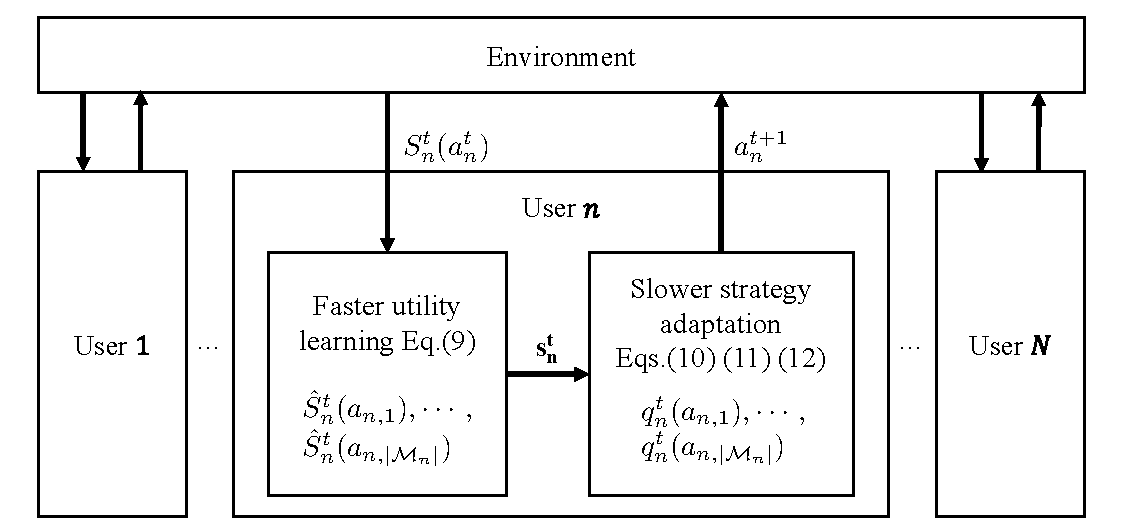
\includegraphics[scale=0.76]{./pic/scheme2.pdf}
%\caption{Illustration of the coupling of utility learning (on faster timescale) and strategy adaptation (on slower timescale) at time $t$.}\label{fg:scheme}
\caption{$t$时刻时效用学习与策略学习之间耦合关系的示意图}\label{fg:scheme}
\end{figure}
我们使用图\ref{fg:scheme}来进一步说明在任意时间步长$t$内效用学习与策略学习之间的耦合。简而言之,在提出的基于遗憾度量的双时间尺度学习算法中,用户在对其长期社交群体效用进行学习的同时,同步地进行策略上的迭代以调整到具有较高“遗憾”度量的信道选择上。在每次迭代中,每个用户都使用其维护的平均遗憾矩阵来计算瞬时遗憾度量(计算复杂度为$O(|\mathcal{M}_n|)$)。接下来,我们对于所提出的学习算法的收敛性能进行评估。
%For clarification, we use Fig. \ref{fg:scheme} to illustrate the coupling of the two learning processes at an arbitrary time step $t$. Simply put, in the proposed regret-based two-timescale learning algorithm, users synchronously learn their long-term group utilities in parallel to the adaptation of their strategies in favor of channels with higher `regret'. At each iteration, each user makes use of her maintained average regret matrix to calculate the instantaneous regret measure, leading to a computational complexity of $O(|\mathcal{M}_n|)$. Next, we evaluate the convergence performance of our proposed learning algorithm.
\vspace{-0.2cm}

\subsection{收敛性分析}\label{sec:conv}

在本节中,我们分析算法\ref{alg:RCS}的收敛性能。我们算法的核心思想是令效用学习和基于无悔学习的策略调整在不同的时间尺度上平行地进行,从而使在较大时间尺度上运行的策略学习可以视在较小时间尺度上运行的效用学习为准静态。我们将采用标准随机逼近理论在双时间尺度上的拓展来证明博弈$\Gamma$对于相关均衡集合的弱收敛性。以下定理给出了我们的主要结果。
%In this section, we analyze the convergence behavior of Algorithm \ref{alg:RCS}. We resort to the two-timescale extension of standard Stochastic approximation theory to show the weakly convergence of game $\Gamma$ to the set of correlated equilibria. The idea is to let the utility learning and regret-based strategy adaptation proceed simultaneously with different step-size schedules so that the regret-based strategy learning runs on a slower effective timescale and sees the utility learning as quasi-static. Our main result is given in the following theorem.
\begin{as}\label{as1}
对于每一个用户$n\in\V$,满足以下条件\textbf{C1-C3},
%For each user $n\in\V$, the conditions \textbf{C1-C3} are satisfied,
\vspace{-0.2cm}
\begin{align}
&\textbf{C1}:\lim_{t\rightarrow\infty}\sum_{t\geq0}\lambda^t_n=+\infty,~\lim_{t\rightarrow\infty}\sum_{t\geq0}(\lambda^t_n)^2<+\infty.\\
&\textbf{C2}:\lim_{t\rightarrow\infty}\sum_{t\geq0}\epsilon^t_n=+\infty,~\lim_{t\rightarrow\infty}\sum_{t\geq0}(\epsilon^t_n)^2<+\infty.\\
&\textbf{C3}:\lim_{t\rightarrow\infty}\frac{\epsilon^t_n}{\lambda^t_n}=0.
\end{align}
\end{as}
\vspace{-0.3cm}
\begin{thm}(算法\ref{alg:RCS}的收敛性)\label{thm:conv}
令$f^t\in\Delta\mathcal{M}$为式(\ref{eq:empi})中定义的经验分布。在满足假设\ref{as1}且式(\ref{eq:reg2})中$\epsilon^t=1/t$的条件下,算法\ref{alg:RCS}收敛到博弈$\Gamma$的相关均衡(CE)的集合$\{\p^*\}$,其中$\pi^*=(\pi^*_1,\pi^*_2,\cdots,\pi^*_N)\in\Delta\mathcal{M}$。特别的,我们有
%Let $f^t\in\Delta\mathcal{M}$ be the empirical distribution as defined in (\ref{eq:empi}). With $\epsilon^t=1/t$ in (\ref{eq:reg2}) and Assumption \ref{as1} being satisfied, Algorithm 1 converges almost surely to the set of CE $\{\p^*\}$ of the game $\Gamma$ with $\pi^*=(\pi^*_1,\pi^*_2,\cdots,\pi^*_N)\in\Delta\mathcal{M}$. In particular, we have,
\begin{align}\label{sne}
&\lim_{t\rightarrow\infty}\hat{S}^t_n(a_{n,i})=\bar{S}_n(a_{n,i},\p^*_{-n}),~\forall n\in\mathcal{M}athcal{V},~\forall i=1,\cdots,|\mathcal{M}_n|,\\
&\mathcal{M}box{and}~~f^t\xrightarrow[\text{}]{\text{a.s.}}\{\pi^*\}~\mathcal{M}box{as}~t\rightarrow\infty.
\end{align}
其中$\bar{S}_n(a_{n,i},\p^*_{-n})$是当用户$n$选择决策$a_{n,i}$,其他用户联合策略为$\pi^*_{-n}$时的期望社交群体效用。
%where $\bar{S}_n(a_{n,i},\p^*_{-n})$ is the expected group utility of user $n$ with action $a_{n,i}$ and others' strategies $\pi^*_{-n}$.
\end{thm}

%\textbf{Outline of the proof.}
定理证明的主要思想是首先引入离散学习过程(\ref{estimation})和(\ref{eq:reg2})的连续时间插值过程。首先,每个学习过程在数学上分别对应于一个微分包含(differential inclusion)\cite{Yin}。而其连续时间差值过程可被证明为对应的微分包含的半流渐近伪轨迹(asymptotic pseudotrajectory of the semiflow)。因而,我们可以通过微分包含来研究序列$\{S_n(\A)\}$和$\{\pi(\A)\}$的极限行为。在满足假设\ref{as1}的前提下,通过结合异步随机逼近框架\cite{Borkar1997},我们可以获得两个并行的学习过程的渐近弱收敛结果。由于篇幅所限,我们在线附录\ref{pf:thm:conv}部分提供详细的证明。
%The main idea of the proof is to first introduce the continuous time interpolated process of the discrete learning process (\ref{estimation}) and (\ref{eq:reg2}), which can be shown to be the asymptotic pseudotrajectory of the semiflow corresponding to the differential inclusion defined by the two learning dynamics\cite{Yin}. Thus the limiting behaviors of the sequences $\{S_n(\A)\}$ and $\{\pi(\A)\}$ can be studied via the differential inclusion. By combining the asynchronous stochastic approximation framework \cite{Borkar1997}, and under the Assumption \ref{as1}, we can obtain the asymptotic weak convergence result of the two concurrent learning processes. Due to the lack of space, we leave the detailed proof to the online appendix \cite{MY18}.

%\vspace{-0.2cm}
\section{性能评估}\label{sec:simulation}
在本节中,我们评估了用于隐私保护下频谱共享的双时间尺度分布式学习算法的性能。
%In this section, we evaluate the performance of the proposed two-timescale distributed learning algorithm for the privacy-preserving spectrum sharing.
%\vspace{-0.4cm}
\subsection{仿真设置}
我们考虑一个数据库辅助的频谱接入网络,该网络由$N=80$个次级用户组成,我们假设这些用户随机分布在$1km \times 1km$的正方形地理区域中。每个用户$n$对应于一个有数据发送需求的移动设备,其默认传输功率为$P_n=100$ mW\cite{FCCApril52012}。我们假设每个用户的可用信道集合即为总的可用信道集合,即$\mathcal{M}_n=\mathcal{M}athcal{A}$,并设置默认的信道总数为$M=5$。我们考虑瑞利信道衰落模型,其中用户$n$和$m$之间的信道增益反比于他们之间的物理距离(路径损耗因子$\alpha = 4$)。我们令$N_{a_n}$表示用户$n$使用信道$a_n$时的背景干扰功率,并假设其数值服从区间[-100,-90] dBm上的均匀分布。我们假设所有的用户被随机分到两个社交群体中,每个群体中用户$n$的权重因子$e_{n}$从均匀分布$\mathcal{M}athcal{U}(e_{min},1)$采样获得,并且设置$e_{min}$的默认值为0.5。
%We consider a database-assisted spectrum access network consisting of $N=80$ IoT devices that are randomly scattered in a square area of 1 km $\times$ 1 km and are categorized into either one of two groups with equal probability. For each secondary user $n$, we set the transmission power before being perturbed as $P_n=100$ mW \cite{FCC} and the available channel set $\mathcal{M}_n=\mathcal{M}athcal{A}$ with $M=5$ by default. We consider a Rayleigh fading channel environment where the channel gain between user $n$ and $m$ is inversely proportional to their physical distance powered by the path-loss factor $\alpha=4$. The background interference power $N_{a_n}$ for each user $n$ using channel $a_n$ is uniformly assigned in the interval of [-100,-90] dBm. The weight factor $e_{n}$ for each user $n$ in either group is generated following a uniform distribution $\mathcal{M}athcal{U}(e_{min},1)$ with $e_{min}=0.5$ by default.
如节\ref{sec:privacy-model}中所述,我们的设计中每个用户通过对其传输功率进行随机扰动以对抗基于RSS的定位攻击。功率扰动程度越大,对于攻击者定位准确性的影响越显著,继而对于位置隐私的保护作用越好。在实验中,我们使用功率扰动的期望值$E(\Delta p_n)$来量化隐私保护程度的大小。
根据式(\ref{eq:noise}),我们可以得出功率扰动项的期望值的表达式为$E(\Delta p_n)=b\left[\frac{1-(k+1)\exp(-k)}{1-\exp(-k)}\right]$,其中$k=\bar{p}/b>0$。我们固定$\bar{p}=15$ mW并默认设置$b=12$,以使平均功率扰动水平约为-6mW。
对于前文提出的双时间尺度学习算法\ref{alg:RCS},我们分别设置学习率为$\lambda^t=t^{-0.5}$和$\epsilon^t=t^{-0.2}$。在满足条件\textbf{C1-C3}的前提下,我们通过网格搜索确定超参数的取值。对于参数$\rho$,我们使用与文献\cite{Hart_areinforcement}中同样的设置,即$\rho=1/8$。
%In our experiment, we let each user randomly perturb her transmission power level to combat the RSS based localization attack (as introduced in Section \ref{sec:privacy-model}), where each user's privacy protection level is quantified by the expected value of power perturbation $E(\Delta p_n)$. According to (\ref{eq:noise}), we can derive the expression for the expected value of power perturbation term as $E(\Delta p_n)=b\left[\frac{1-(k+1)\exp(-k)}{1-\exp(-k)}\right]$, where $k=\bar{p}/b>0$. We fix $\bar{p}=15$mW and set $b=12$ by default such that the mean perturbation level is about -6mW.
%For the two-timescale learning algorithm, we set the learning rate $\lambda^t=t^{-0.5}$ and $\epsilon^t=t^{-0.2}$ in Algorithm 1. The value of hyperparameters are determined through a tuning process so that the conditions \textbf{C1-C3} are satisfied. In addition, we let $\rho=1/8$ as it is used in \cite{Hart_areinforcement}. 

%\vspace{-0.2cm}
\subsection{结果与讨论}
\subsubsection{收敛表现}
我们首先检查算法的收敛性能。在默认设置$E(\Delta p_n)=-6$ mW,$e_{min}=0.5$的条件下,我们针对不同数量的可用信道集合进行实验,即$M=4,5,6$。我们使用网络吞吐量$T=\frac{1}{N}\sum_{n\in\mathcal{M}athcal{V}}T_n$作为性能指标,其中$T_n$表示用户$n$的平均吞吐量。从图\ref{fg:conv1}中我们观察到算法在1500次迭代内可以收敛,而通道总数的增加会导致收敛时间的增长。同时可以看出,系统可实现的最大网络吞吐量大约占网络吞吐量最优值的90%,且并不会受到信道集合大小变化的影响。图\ref{fg:conv2}则分别展示了任意选择的一个用户(\#10)所对应的每一个信道的策略的收敛性表现。
%We first examine the convergence performance of our algorithm. We adjust the value of $b$ so that the mean value of power perturbation magnitude is -5 mW and the minimum group-relationship strength $e_{min}=0.5$. We first run the experiment with different number of available channels, $M=4,5,6$. The network throughput $T=\frac{1}{N}\sum_{n\in\mathcal{M}athcal{V}} T_n$ is used as the performance metric, where $T_n$ denotes the average throughput of user $n$. From Fig. \ref{fg:conv1}, we observe that the proposed algorithm converges within 1500 iterations in general with increased number of channels leading to longer convergence time. It can be observed that changing the size of channel set does not impact the maximum achievable network throughput, which accounts for about 90\% of the optimal network throughput. For an arbitrary selected user \#10, we further evaluate the convergence of her strategies over each of the available channels, as shown in Fig. \ref{fg:conv2}.
%\begin{figure}[htb]
%\centering
%\subfloat[]{
%	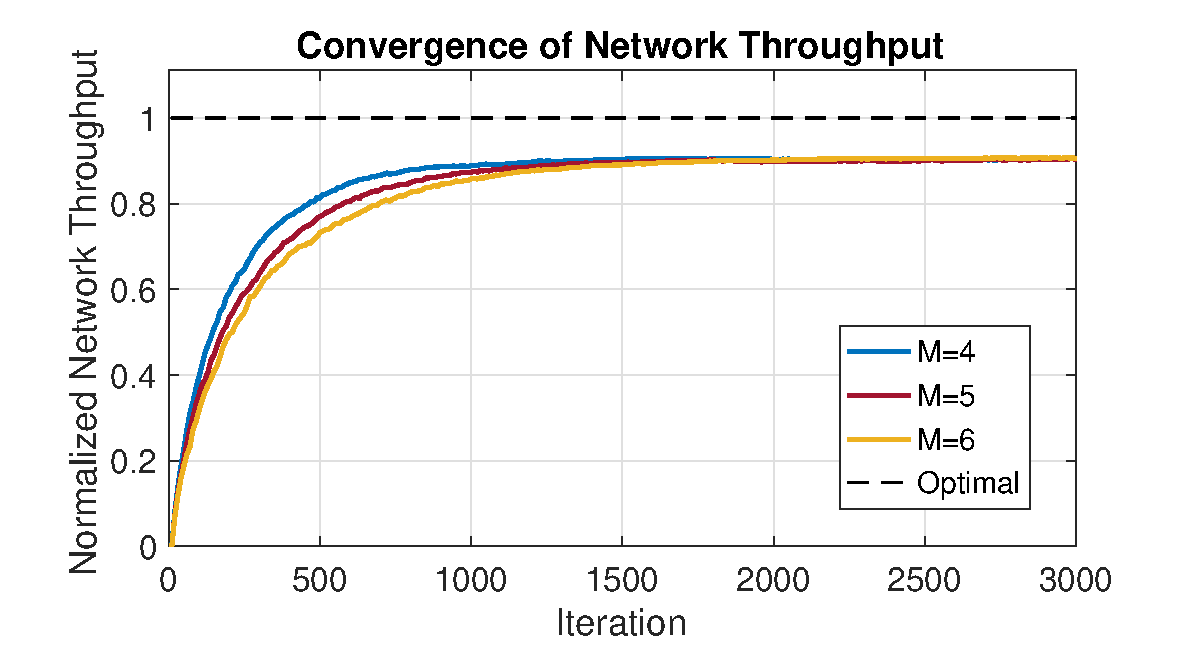
\includegraphics[scale=0.41]{./pic/conv_ch3.eps}\label{fg:conv1}}
%\vfill
%%\vspace{-0.3cm}
%\centering
%\subfloat[]{
%	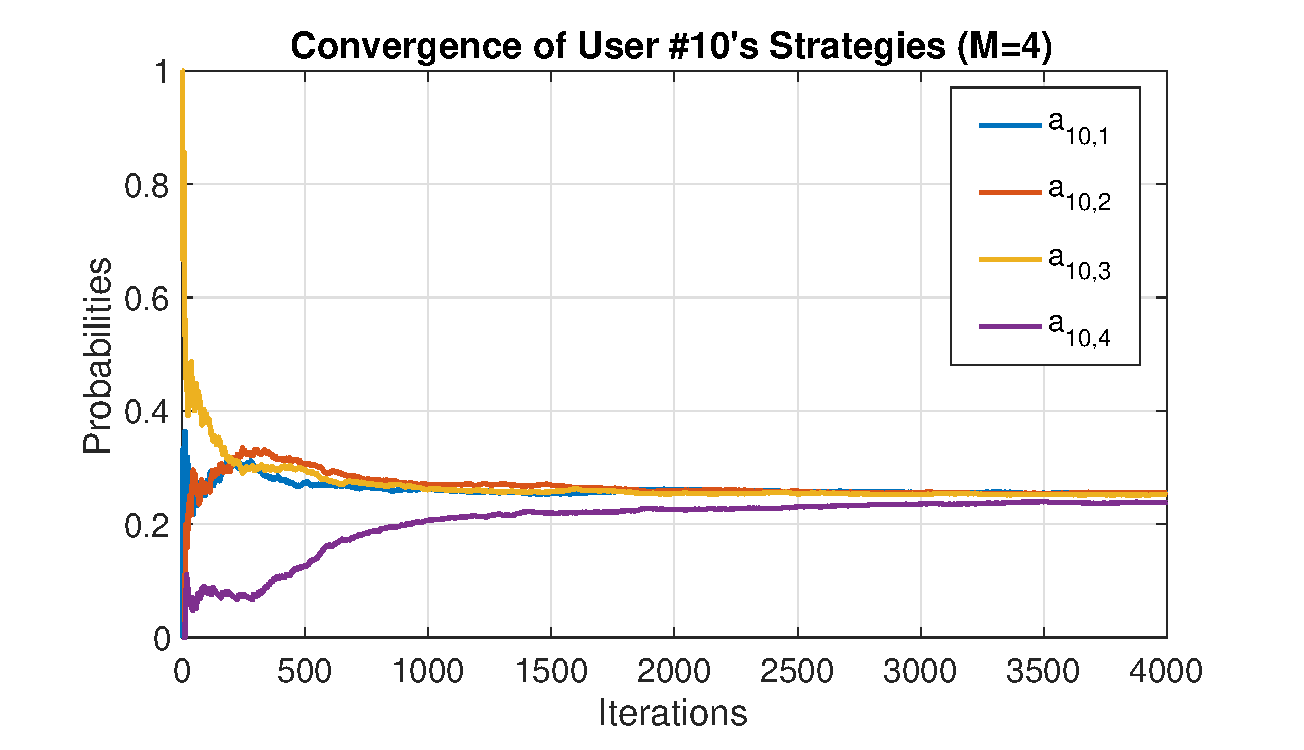
\includegraphics[scale=0.4]{./pic/str_conv4.eps}\label{fg:conv2}}
%%\hfill
%\caption{Convergence performance of two-timescale distributed learning algorithm.}\label{fg:Fig11}
%\end{figure}

%\begin{figure*}[!t]
%	\begin{minipage}[t]{0.48\textwidth}
%		\centering
%		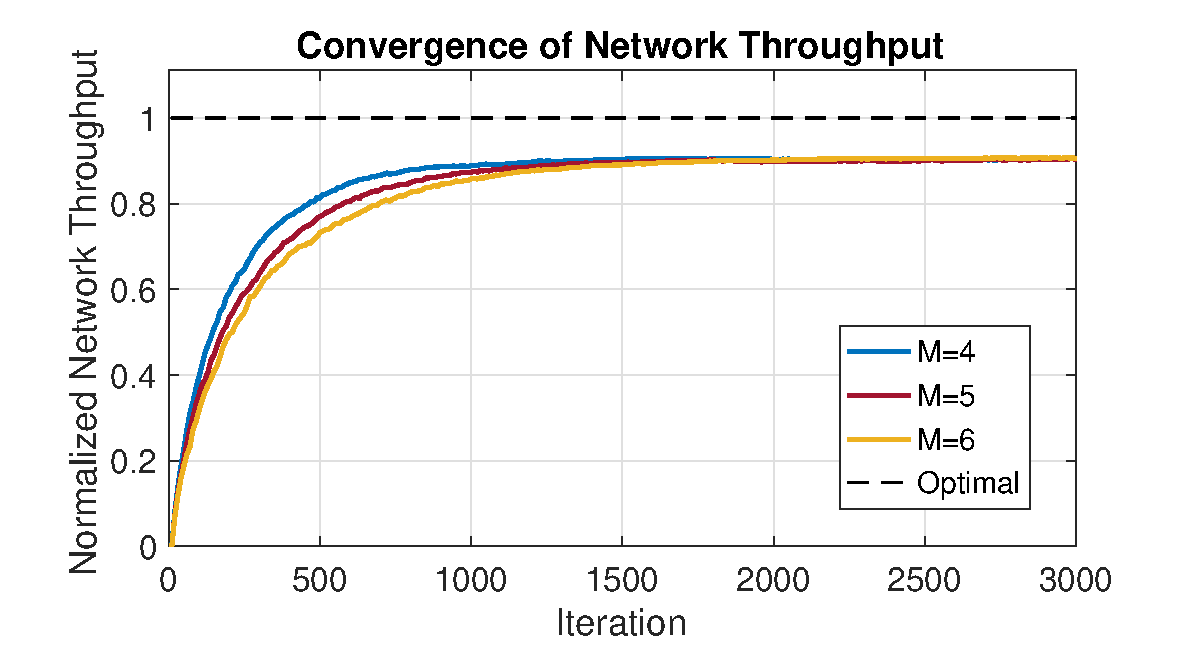
\includegraphics[scale=0.44]{./pic/conv_ch3.eps}
%		\caption{网络吞吐量的收敛表现}\label{fg:conv1}
%	\end{minipage}
%	\hfill
%	\begin{minipage}[t]{0.48\textwidth}
%		\centering
%		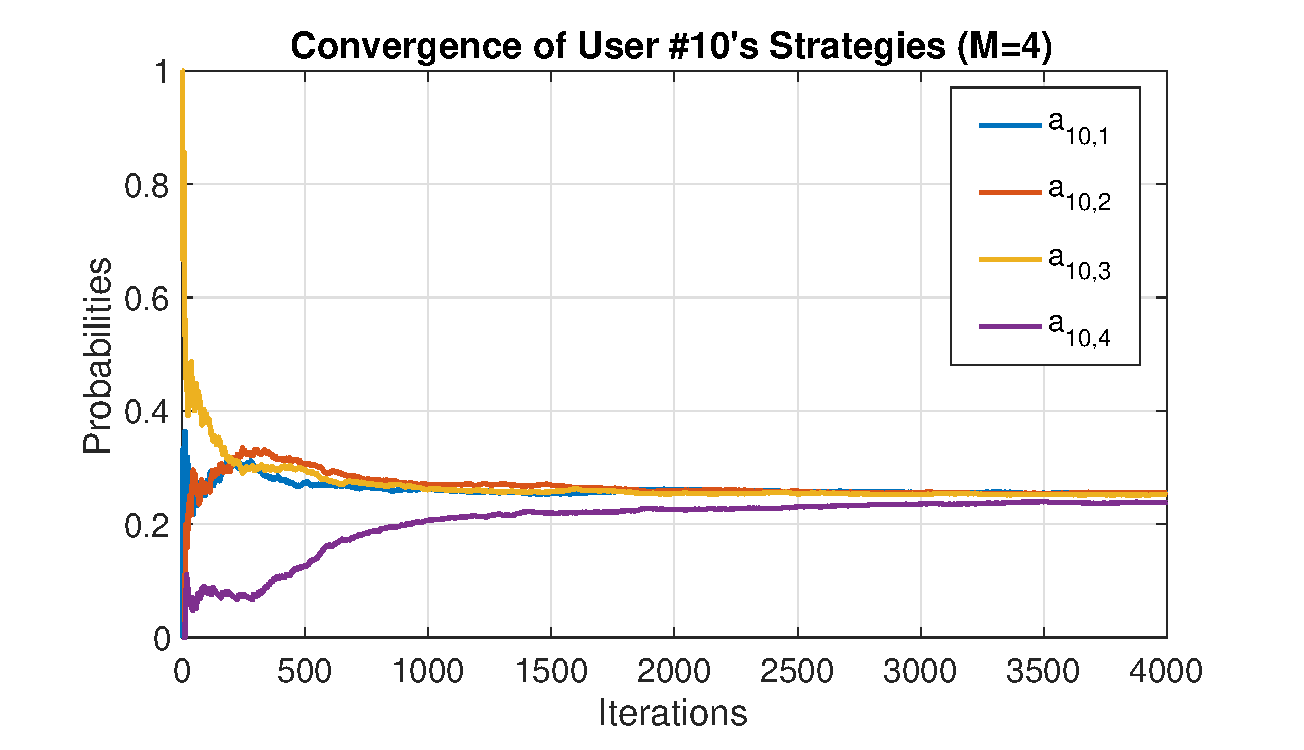
\includegraphics[scale=0.42]{./pic/str_conv4.eps}
%		\caption{用户\#10的策略收敛表现 (M=4)}\label{fg:conv2}
%	\end{minipage}
%	\caption{双时间尺度分布式学习算法的收敛性表现}
%	\label{fg:Fig11}
%\end{figure*}

\begin{figure*}[!t]
%	\begin{minipage}[t]{0.48\textwidth}
		\centering
		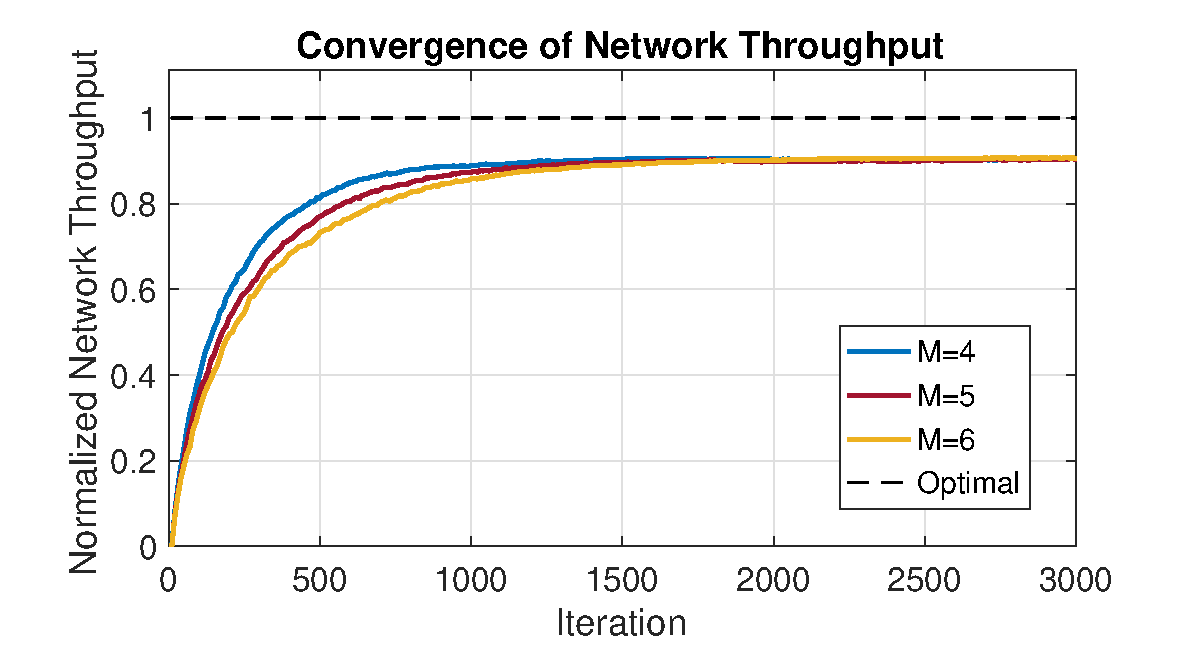
\includegraphics[scale=0.65]{./pic/conv_ch3.eps}
		\caption{网络吞吐量的收敛表现}\label{fg:conv1}
\end{figure*}
%	\end{minipage}
%	\hfill
%	\begin{minipage}[t]{0.48\textwidth}
\begin{figure*}[!t]
		\centering
		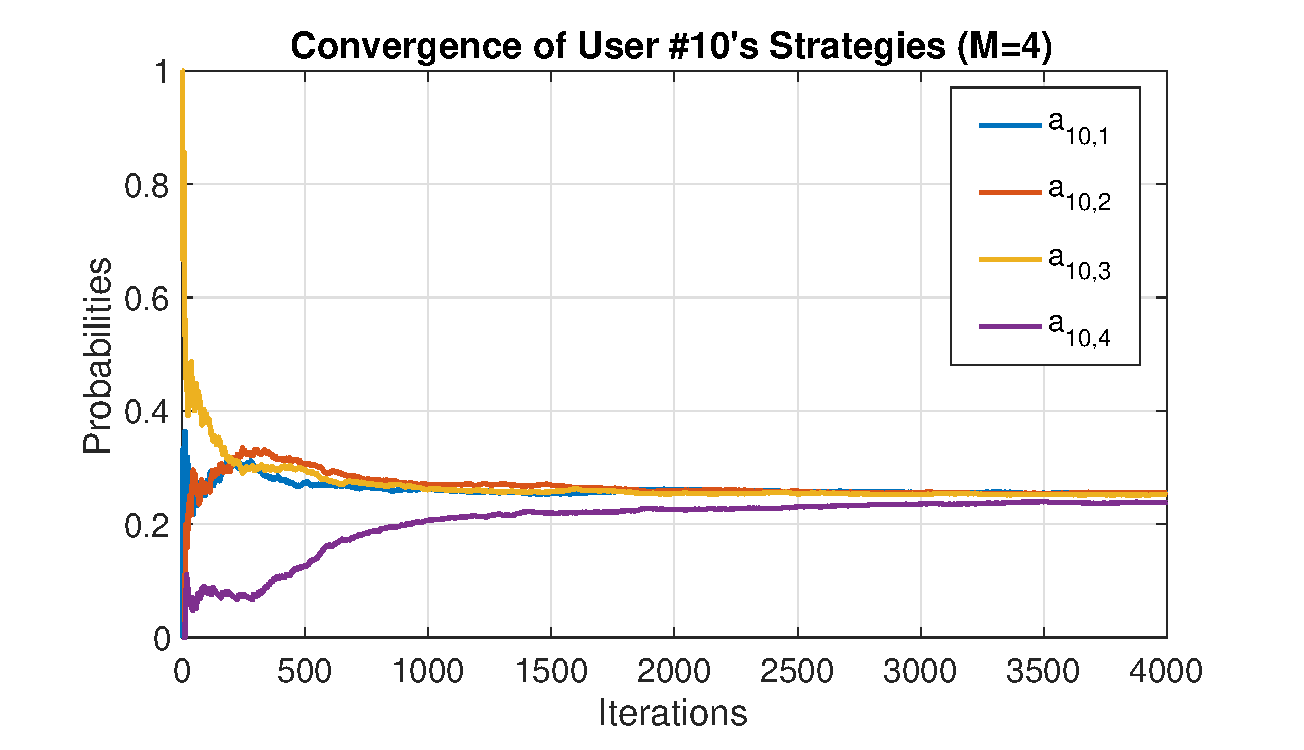
\includegraphics[scale=0.64]{./pic/str_conv4.eps}
		\caption{用户\#10的策略收敛表现 (M=4)}\label{fg:conv2}
%	\end{minipage}
%	\caption{双时间尺度分布式学习算法的收敛性表现}
%	\label{fg:Fig11}
\end{figure*}



\subsubsection{关于吞吐量-隐私权衡的比较性实验}
%\subsubsection{Comparative studies on the throughput-privacy tradeoff}
我们接下来研究在不同功率扰动水平下网络吞吐量与位置隐私之间的权衡。我们使用默认设置$M = 5$,$e_ {min} = 0.5$,并在不同功率扰动级别下运行实验。具体来说,我们通过更改参数$b$的值,使得扰动功率的平均值在0mW至-9mW之间变化。为了进行比较研究,我们考虑了两个基准:(a)单一时间尺度学习算法,该算法仅使用\ref{sec:single}节中所介绍的修正后的无悔学习规则进行策略上的调整而不引入对于效用的学习; (b)双时间尺度学习算法,其中包括在较小时间尺度上对于效用的学习以及在较大时间尺度上使用随机虚拟对弈(Stochastic Fictitious Play)\cite{ZhangGlobe}进行策略调整。

%We next investigate the tradeoffs between network throughput and location privacy under different levels of power perturbation. We use the default setting of $M=5$, $e_{min}=0.5$, and run the experiment under different levels of power perturbation. Specifically, we change the value of parameter $b$ so that the mean value of perturbation power level varies from 0mW to -9mW. For the comparative study, we consider two benchmarks: (a) the single timescale learning algorithm that merely consists of strategy adaptation based on modified regret based learning (RBL) as introduced in Section \ref{sec:single}; (b) the two-timescale learning algorithm involving a utility learning as well as a strategy adaptation following the Stochastic Fictitious Play (SFP) \cite{ZhangGlobe}. 

如图\ref{fg:Fig33}所示,正如所预期的,系统吞吐量会随平均功率扰动水平的增加而降低。同时,很明显,使用单一时间尺度的学习算法在隐私保护级别升高时,网络吞吐量较其他两种算法相比下降得更快。这表明引入平行的效用学习来校准带有噪声的效用观测值的有效性。这也有助于我们可以在位置隐私保护与保证网络性能(即系统吞吐量)之间取得权衡。
%As shown in Fig. \ref{fg:Fig33}, in general, the system throughput decreases as expected with the increase of mean power perturbation level. Meanwhile, it is clear that the throughput of single timescale learning using RBL degrades much faster as the privacy preserving level increases, compared with other two approaches that involve both utility learning and strategy adaptation. This indicates the effectiveness of using a parallel utility learning to calibrate the noisy utility observation, which helps balance the location privacy protection with the network performance (i.e., system throughput). 

从图\ref{fg:Fig33}中还可以看出,我们所提出的基于无悔学习的双时间尺度算法所获得的平均吞吐量比使用\cite{ZhangGlobe}中提出的双时间尺度学习方法所获得的平均吞吐量平均要高5%。这样的结果可以由两种方案中所使用的不同均衡标准来解释。文献\cite{ZhangGlobe}中提出的算法针对的是纳什均衡。根据定义,纳什均衡假设博弈参与者的策略之间是相互独立的,而本研究中所考虑的相关均衡则允许参与者的策略之间存在相关性,因此相比纳什均衡更具一般性。由于相关平衡的集合在数学上等价于一个凸多胞形,并且凸多胞形的每一个极值点即对应于一个纳什均衡点,因此一般而言以相关均衡为考虑对象可以使得结果展现出更好的性能。
%It can also be seen that the throughput obtained by our proposed algorithm outweighs the one obtained using the two-timescale learning approach introduced in \cite{ZhangGlobe} by 5\% in average. This can be explained by the different  Equilibrium criteria used in the two studies. By definition, Nash equilibrium uses an underlying assumption that players' strategies are mutually independent. While the correlated equilibrium considered in this study generalizes the Nash equilibrium by allowing the strategies to be dependent among players. As the correlated equilibrium is mathematically equivalent to a convex polytope with its extrema points corresponding to the set of Nash equilibria, it is likely to exhibits better performance in general. 
\begin{figure}[htb]
\centering
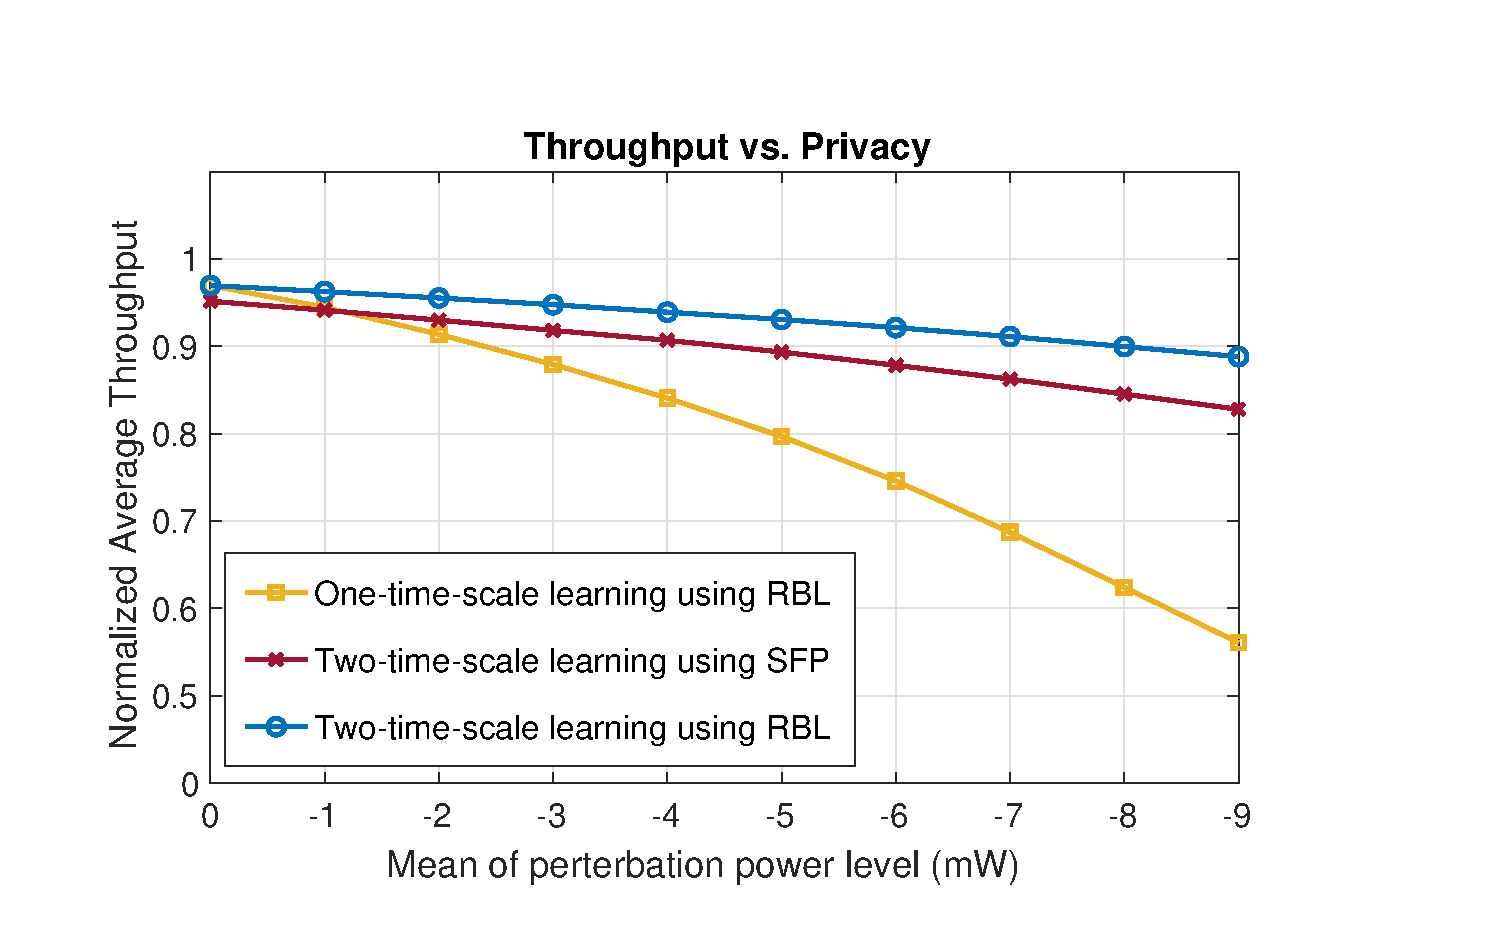
\includegraphics[scale=0.58]{./pic/thp_pert_new3.eps}
%\vspace{-0.0cm}
%\caption{Performance comparisons among different learning algorithms under varying power perturbation level.}
\caption{几种学习算法在不同功率扰动水平下的性能比较}\label{fg:Fig33}
\end{figure}
%\vspace{-0.2cm}
\begin{figure}[htb]
\centering
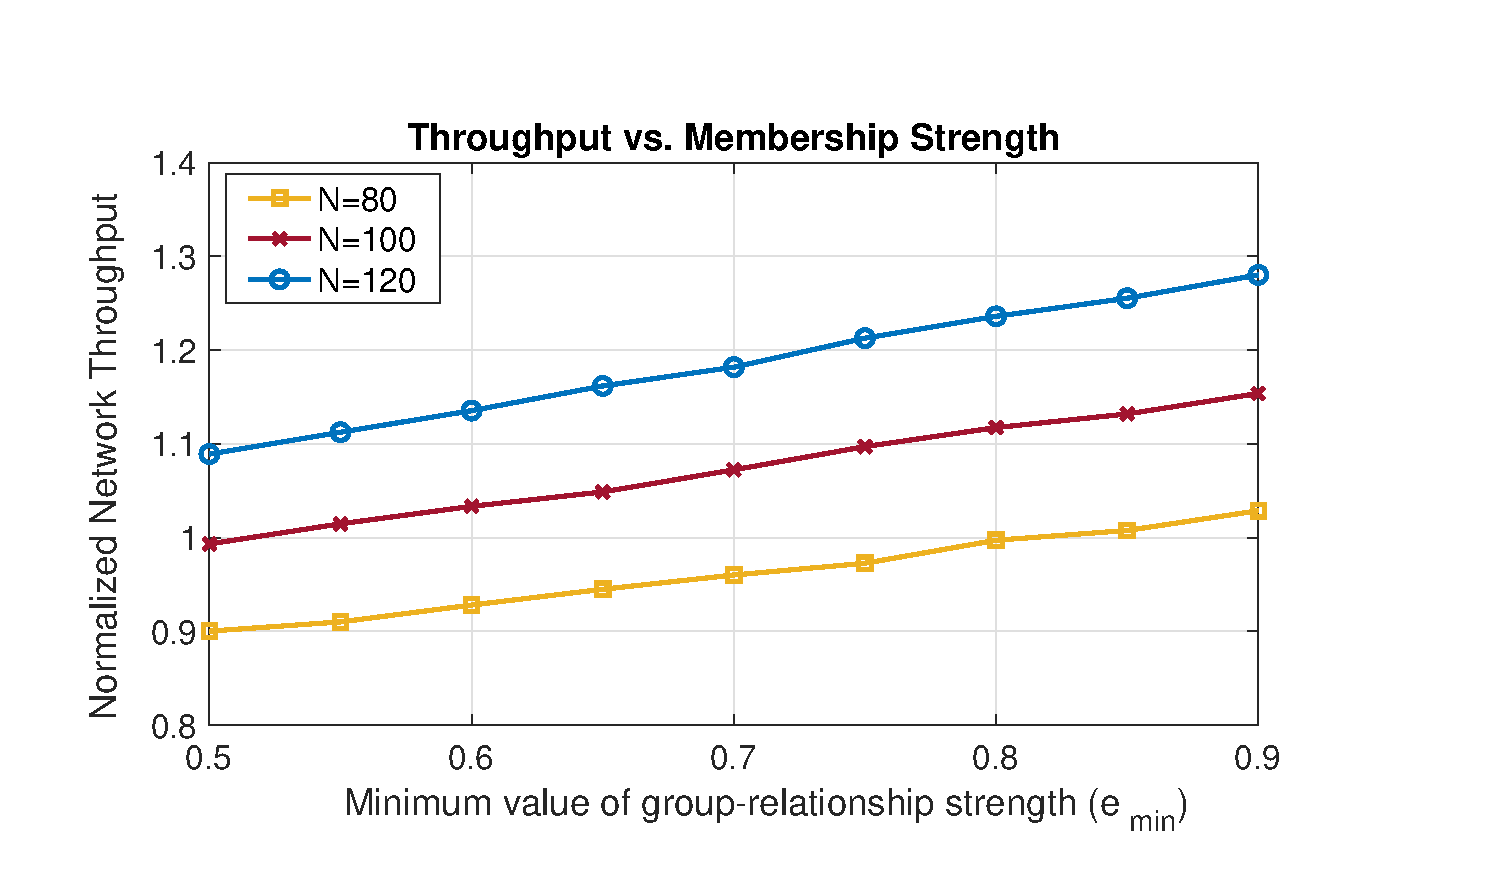
\includegraphics[scale=0.58]{./pic/thp_soc_new3.eps}
%\vspace{-0.3cm}
\caption{社交联系强度对吞吐量的影响}\label{fg:Fig22}
\end{figure}
\subsubsection{网络外部性对于系统吞吐量的影响} 我们最后对网络外部性对系统性能的影响进行评估。实验中我们分别针对三种网络规模(即$N = 80, 100, 120$)在将社交关联强度参数$e_ {min}$取值从0.5增加到0.9的过程中对系统的吞吐量进行了考察。如图\ref{fg:Fig22}所示,随着系统规模的扩大,网络吞吐量呈逐步增长的趋势。另外,可以看出,系统吞吐量会随着社交关联强度的增加而单调增加。具体的,对于$N = 80, 100, 120$的三种情况,当$e_ {min}$从0.5增加到0.9时,系统性能分别可以获得大约14.5%,15%和16.4%的提升。这说明正向的网络外部性影响有助于提升系统的表明。
%We finally examine the network impact to the system performance. We run the experiment with increasing $e_{min}$ from 0.5 to 0.9 for three cases with different network scale, i.e., $N=80, 100, 120$. As illustrated in Fig. \ref{fg:Fig22}, the network throughput grows in general as the system scale enlarges. Also, it can be seen that the throughput experiences a monotonically increase as the strength of in-group relationship increases. For the cases with $N=80, 100, 120$, approximately 14.5\%, 15\%, and 16.4\% performance gains are achieved, respectively, when $e_{min}$ is increased from 0.5 to 0.9, which indicates that the system would benefit from users behaving more altruistically. 

%\vspace{-0.2cm}
\section{本章小节}\label{sec:con}
本章关注了认知无线电网络中的数据库辅助频谱共享技术,其中次级用户在双重网络外部性的作用下分别在社交域和物理域中都存在相互耦合。针对潜在的基于RSS的位置隐私攻击,次级用户使用随机功率扰动的方法来降低攻击者的定位精度。本文将隐私保护下具有社会意识的频谱共享建模为次级用户之间的随机信道选择博弈。基于无悔学习的规则,本文设计了一种双时间尺度的分布式学习算法。算法中,每个用户持续对自己带有噪声的期望社交团体效用进行估计,并根据降低遗憾度量的目标调整其信道选择策略。本文所提出的算法具有针对相关均衡集合的弱收敛性。数值结果证实较高的隐私保护级别将导致更严重的网络吞吐量下降。
%In this paper, we studied database assisted spectrum sharing where secondary users are coupled both in the social domain and in the physical domain. To address the RSS-based location privacy attack, a random power perturbation approach is applied to reduce the localization accuracy. We cast the socially-aware privacy-preserving spectrum sharing as a stochastic channel selection game among secondary users. Based on no regret dynamics, we develop a two-time-scale distributed learning algorithm in which each user continuously estimates her social group utility and adapts her strategy in favor of reduced regrets. Our algorithm is shown to weakly converge towards the set of correlated equilibrium. The numerical results corroborate that higher privacy protection level would lead to severer network throughput degradation.

